%!TEX root = project.tex

\chapter*{About this project}
\paragraph{Abstract}

This project will help to explain the temporal difference reinforcement learning process by displaying an agent's behaviour, performance and Q-Table (memory) as it interacts within its environment. The application is a browser based visual tool where a user can tweak parameters within a form before running the application. Once the form is submitted, it will then make a request to run the application held on a server. Once the script has completed, the user will be presented with and animation of the agent moving through it's environment. In addition, a graph of the agent performance and the q-table will presented to the user for examination. There are two different temporal difference algorithms for the user to choose being Q learning, an off policy strategy and SARSA (State Action Reward Action), an on policy strategy. The performance of these two algorithms will be presented to the user for examination within a linear chart.
This will aid the user in better understanding the concept of reinforcement learning.

\paragraph{Authors}
Kevin Gleeson, 4th year student studying Software Development at GMIT Galway.



\chapter{Introduction}
\textbf{Reinforcement learning}\\
\begin{figure}[H]
	\centering
	\includegraphics[width=0.7\linewidth]{"../../../Project Plan/grid_world_env"}
	\caption{Image Source~\cite{GridWorl45:online}}
	\label{fig:gridworldenv}

\end{figure}
Reinforcement Learning is an unsupervised machine-learning technique that allows an agent to explore and learn from its environment without any prior knowledge of the domain. 
An agent transitions from one state to another by choosing an action with the highest reward value. The reward can be either positive or negative, based on the decisions made by the agent, as it transitions from it's current state to the next chosen state.\\
For example, if a puppy has no knowledge of the sit command, it will not perform the desired action on the first attempt. Each time the puppy sits when commanded, its decision is reinforced with a positive treat/reward. If the puppy does not sit, the reward is negative (no treat). Eventually after many iterations of training, the dog will associate a treat/reward with that specific command and eventually learn that sitting will get them a treat. 
The puppy, in essence, is taking actions to maximise rewards while exploring an unknown environment.\\
With reinforcement machine learning, the technique is used to train an agent to learn about its environment through trial and error. It will eventually learn the optimal path to a goal after many training episodes have been completed.

\section{Components}
This application will have the following reinforcement learning components.

\section{Markov Decision Process}
The Markov decision process has the requirement of being in a present state all future states are independent of past states.\\\\
$P[S_{t}+1 | S_{t}] = P[S_{t}+1 | S_{1}, ..... , S_{t}]$\\\\

The above equation simply states that the current state holds all of the past cumulative values where future actions can be decided.
Where $P$ is the probability of taking a future action $St+1$  from a current state $St$. Therefore there is no need to keep track of the entire history of the actions taken for every state. The Markov decision process is used in reinforcement learning to allow the agent to only observe it's current state and choose a future action based on the total reward values from previous states observed~\cite[p.~67]{sutton_barto_2018}.

\section{Bellman Equation}
$V(s) = max_{a}(R(s,a)+\gamma V(s'))$\\\\

The Bellman equation is used in conjunction with the Markov decision process where $V$ is a value function, $a$ is an action taken, $R$ is the reward gained, $(s,a))$ represents the state and action taken, $\gamma$ is the discount factor $(s')$ is the next state~\cite[p.~75]{sutton_barto_2018}.
\\

This is a recursive function where the maximum reward for the current state and action is assigned to the next state. A discount factor is applied where the future cumulative rewards are assigned. The closer gamma is to the value one, the updated value will be directly related to the adjacent state. With a gamma value closer to zero it will take into consideration the future rewards for the next n states.
\subsection{Agent}
The agent is an object within the environment that makes decisions based on it's current state space and possible rewards gained by choosing an action. For this application, the agent is placed in a two dimensional environment. The possible actions that can be taken by the agent are up, down, left or right~\cite{nwana_1996}.\\
\subsection{Episode}
An episode is the time from when an agent starts its training to when it has reached a positive or negative terminal state. Within each episode an agent takes time steps where each time step is the transition from its current position to the next within the environment~\cite{Watkins1992}.
\subsection{Environment}
The environment used for this project will be grid world. The grid world domain is a two dimensional grid with the agent's start position at the bottom left of the grid and the goal state at the top right of the grid. In addition there are traps that the agent needs to avoid while travelling from the start state to it's goal state.
For the purpose of this application a  6 * 6 two dimensional grid environment will be used. As the script is running the agent will move from one square in the grid to the next adjacent square of up, below, to the left or the right of its current position. As the agent moves through the environment it gains knowledge via reward signals gathered by transitioning from one state to another based on the action taken from its current state.
\subsection{Epsilon}
The Epsilon variable sets the probability of choosing a random action. When set to one, it will always choose a random action. If set to .8 it will choose the a random action 80\% of the time. This value is decayed for every episode run to allow for the exploration of the environment~\cite{LITTMAN1994157}.
\subsection{gamma}
The discount factor (Gamma) set to .9 is the immediate reward gained for an action taken. The discount factor is a values between zero and one. The higher the value the more the agent will take an immediate reward with no concern for future rewards~\cite{LITTMAN1994157}.
\subsection{alpha}
The learning rate (alpha) is a value between zero and one that determines how much a Q value is updated for each action taken. It will be .5 for this example. The closer the value is to one the quicker the agent will learn, however it may not take into consideration other possibilities that may eventually lead to a greater reward. A lower learning rate is considered the optimal setting, where the agent gradually draws a numeric picture from its entire environment, rather than just gathering information from its immediate state~\cite{LITTMAN1994157}. 
\subsection{per step cost}
There is a negative reward cost for each step the agent makes in this case -0.04.
This reward is cumulative and  added to the final reward the agent gains at the end of each episode. This will help in getting the best path to the end state~\cite{LITTMAN1994157}.
\subsubsection{Q Values}
 Q values are a weighted score attached to an action of up, down, left or right for a particular state.
 The agents next movement is based on theses weighted scores. With the action taken usually being the highest possible q value. There is however the epsilon variable discussed above that may effect this~\cite{LITTMAN1994157}.

\subsubsection{Updating Q values}
The agent chooses it's action decision based on what highest reward it can get from the next available states.\\

With the Q Learning algorithm each time step and action taken by the agent the following formula is used to update the Q values within the Q Table. This is considered an off policy optimistic approach as the maximum value from all possible actions in the next state are use to update the current Q value for the agents action taken~\cite{Watkins1992}\\\\
$ Q^{new}(s_{t},a_{t})\leftarrow Q(s_{t},a_{t}) + \alpha[r_{t} + \gamma  \max _{a}Q(s_{t+1},a) - Q(s, a)]$~\cite{Qlearnin52:online}\\\\
This above formula can be broken can be simplified as:\\\\
Q (current state, action) += alpha *[reward + gamma* max value of Q (next state, all possible actions) – Q (current state, action)]\\\\

The SARSA algorithm is considered an on policy pessimistic approach as the Q value is updated from the actual action taken from the current state and the maximum value as Q Learning does. There is just a small difference between the two algorithms but it has a significant impact on the behaviour of the agent. This will be evaluated later in the System Evaluation chapter of this document.\\\\
$Q(s_{t},a_{t})\leftarrow Q(s_{t},a_{t})+\alpha [r_{t}+\gamma Q(s_{t+1},a_{t+1})-Q(s_{t},a_{t})]$~\cite{Stateac29:online}\\\\
This formula can be simplified as:\\\\
Q (current state, action) += alpha *[reward + gamma*  Q (next state, next action) – Q (current state, action)]\\\\



\subsection{Q Table}
The Q table is a historic record of the agent’s actions taken in a given state. The values held within the Q table are used by the agent to choose the next best state transition. During the first episode all values within the Q table are zero (No knowledge of the environment). With every time step taken, the Q table is updated with q values from the above formula. For brevity, the below examples will use a smaller q table rather than the one used for this application.
At the beginning of the learning process the Q Table has all zero values meaning it has no prior knowledge of its domain~\cite{Lanzi2002}.
\\
\\
\begin{tabular}{lllll}
State & Action left & Action right & Action up & Action down \\
1     & 0           & 0            & 0         & 0           \\
2     & 0           & 0            & 0         & 0           \\
3     & 0           & 0            & 0         & 0           \\
4     & 0           & 0            & 0         & 0           \\
5     & 0           & 0            & 0         & 0           \\
6     & 0           & 0            & 0         & 0           \\
7     & 0           & 0            & 0         & 0           \\
8     & 0           & 0            & 0         & 0           \\
9     & 0           & 0            & 0         & 0           \\
10    & 0           & 0            & 0         & 0           \\
11    & 0           & 0            & 0         & 0          
\end{tabular}
\\
\\
From its initial state a random action is chosen. If the action chosen is to move up one square to state 5 the Q table is updated using the q learning formula above which looks like   .5 * -.04  + .9 *0 – 0 = -0.02.
It then populates the Q table's row of State one's action of moving up to the q value of -0.02.

\begin{tabular}{lllll}
State & Action left & Action right & Action up & Action down \\
1     & 0           & 0            & -0.02     & 0           \\
2     & 0           & 0            & 0         & 0           \\
3     & 0           & 0            & 0         & 0           \\
4     & 0           & 0            & 0         & 0           \\
5     & 0           & 0            & 0         & 0           \\
6     & 0           & 0            & 0         & 0           \\
7     & 0           & 0            & 0         & 0           \\
8     & 0           & 0            & 0         & 0           \\
9     & 0           & 0            & 0         & 0           \\
10    & 0           & 0            & 0         & 0           \\
11    & 0           & 0            & 0         & 0          
\end{tabular}
\\
\\
\\
If the Agent decides to move down to state one again the value of moving down from state 5 to state 1 is updated to -0.02 also.
\\

\begin{tabular}{lllll}
State & Action left & Action right & Action up & Action down \\
1     & 0           & 0            & -0.02     & 0           \\
2     & 0           & 0            & 0         & 0           \\
3     & 0           & 0            & 0         & 0           \\
4     & 0           & 0            & 0         & 0           \\
5     & 0           & 0            & 0         & -0.02       \\
6     & 0           & 0            & 0         & 0           \\
7     & 0           & 0            & 0         & 0           \\
8     & 0           & 0            & 0         & 0           \\
9     & 0           & 0            & 0         & 0           \\
10    & 0           & 0            & 0         & 0           \\
11    & 0           & 0            & 0         & 0     
\end{tabular}
\\
\\
When back in state one, the agent’s best choices (highest value) is down, left or right as they are all 0 and higher the -0.02. This happens for every time step the agent takes. When enough episodes have run, all of the actions of a given state will have a value added including the goal state value. From this the agent will chose the highest value each state as the optimal action to take to the end goal. 
Once the agent gets to either end state, the episode is terminated and re-run. When episodes are re-run, the Q-Table will continually update until the optimal path is found and minimal updates will be performed.\\

\begin{tabular}{lllll}
	State & Action left & Action right & Action up & Action down \\
	1     & -0.02           & -0.02              & 0.02     & -0.02           \\
	2     & -0.02           & -0.05            & -0.02         & -0.02           \\
	3     & -0.02           & -23            & -23         & -0.02           \\
	4     & -0.02           & -23            & -100        & -0.02           \\
	5     &  -0.02        & -0.02           & 10       & -0.02       \\
	6     & -75           & -100            & 1.2         & -15           \\
	7     & 0           & 0            & 0         & 0          \\
	8     & 15           & 75            & -0.02         & -0.02           \\
	9     & -0.02          & 85           & -0.02        &-0.02         \\
	10    &  -0.02            & 100            &  -0.02          &  -0.02  \\ 
	11    & 0           & 0            & 0         & 0         
\end{tabular}
\\
\\
The purpose of this application is to demonstrate and explain reinforcement learning through a browser based visualisation tool.\\
The application will have the following elements on the Browser:
\begin{itemize}
\item The agent moving within its environment when the simulation is run.\\This will be displayed using HTML 5 canvas and represented by a yellow square within the canvas.

\item User form input to tweak parameters before each run of the simulation. The parameters that will be available to the user are:
	\begin{itemize}
		\item The end goal reward
		\item The negative trap reward
		\item The agent learning rate
		\item The learning decay rate
		\item The discount factor
		\item The Exploration rate
		\item The Exploration decay rate
		\item The per step reward
		\item The maximum number of episodes to be run
		\item The maximum number of agent steps per episode
		\item Choice of algorithm
	\end{itemize}
\end{itemize}


\chapter{Context}

\section{Overview}
The aim of this project is to provide a visual aid that further explains the concept of reinforcement learning. The basic fundamentals of the Q-Learning and SARSA temporal difference algorithms are reasonably straight-forward but can seem overly complex and verbose when attempting to verbally explain the topic. This application will help the user visualise where and how the Q-values are stored and how the decision making process is made for the two above algorithms.

\section{Objectives}
The Main objectives of this project are:
\begin{itemize}
	\item Implement two different temporal difference algorithms SARSA and Q-learning written in python.
	\item Allow for user interaction via a web page form
	\item Using Flask server to handle request from the user
	\item Present the user with data generated by the main python script on the server 
	\item Parsing Json, text and csv files generated via Ajax
	\item Use the parsed data to animate the agent in HTML canvas
	\item Google chart for graphing the agent performance
	\item Generate an dynamic table that updates from the csv file
	\item Add a heat map to the values of the table as it updates
	\item Deploying the application to Google Cloud Platform

\end{itemize}
 


\section{Topics Covered}
The chapters listed below will have the following elements examined.
\begin{itemize}
	\item Methodology\\
	This chapter will explain what development process I used along with reasoning the technologies, algorithms and languages chosen.
	\item Technology Review\\
	This chapter will review each technological element of the application and provide a justification for each technology discussed.
	\item System Design\\
	The overall architecture will be explained with diagrams of each component of the system supplied.
	\item System Evaluation\\
	The performance of the overall application will be evaluated here. In addition the limitations of the application discovered while in development will be discussed in detail.
	\item Conclusion\\
	In this chapter, the results of the system evaluation will be discussed along with any new findings that may have occurred.
\end{itemize}
\section{Github Repository}
The below link is the url to the github repository holding my dissertation and software files.\\
\href{https://github.com/kevgleeson78/Reinforcement-Learning}{https://github.com/kevgleeson78/Reinforcement-Learning}.
The contents of this repository are:
\begin{itemize}
	\item Dissertation folder\\
	This folder holds the latex files for my dissertation developed using Tex Studio
	\item FlaskApp Folder\\
	This is the main application folder stored on a Flask server when deployed.
	\item FlaskApp / flaskTest.py\\
	This file is used to serve the main static html page and handle http form requests 
	\item FlaskkApp / Environment.py\\
	This file is the main file holding the logic and environment space for the application.\\
	All of the data files are generated from here once run.
	\item FlaskApp / app.yaml\\
	This file is used to deploy the application to a Google Cloud App engine instance.
	\item FlaskkApp / requirements.txt\\
	This file is used to declare what resources are needed fro the application to run on Goolge Cloud
	\item FlaskApp / Static / JavaScript\\
	Each of the files contained within this folder are the main JavaScript files controlling the HTML canvas environment, Google Chart and Q-Table data.
	\item FlaskApp / Static / Css\\
	The folder holding the styling script for the html pages
	\item FlaskApp / Static / gif
	The folder holding the gif animation for the loading page
	\item FlaskApp / Static / Data \\
	The folder holding the agents position coordinates as a .txt file\\
	A csv file for the agents Q-Table values
	A json file for the agent rewards gained for each algorithm
	\item FlaskApp / Templates\\
	This folder contains the the initial html page, the waiting page and result page. These pages are served to the browser view when http requests are made by the client.
	
\end{itemize}

\chapter{Methodology}
\section{Initial Planning}
At the beginning of this project, the over-all problem set was broken down into the following areas to allow for a more manageable modular development process:

\subsection {Initial Meetings}
After an initial meeting with Dr. Patrick Mannion, a high level view of the project was explored. This gave me a grasp of what components would be needed for the high level structure of the project.
The different components identified were:
\begin{itemize}
	\item The Environment should be a two dimensional grid 
	\item Environment constraints are in the form of a grid world game where the agent will attempt to navigate to an end goal state and avoid any traps present in the gird.
	\item Front end technologies used should be JavaScript based.
	\item User interactivity via a from 
	\item Server side functionality to handle form requests
\end{itemize}

On further meetings with my project supervisor Mr. Martin Hynes, the concepts were further broken down into fine grain units of work with initial milestones set for each phase of development.
\subsection {Which area of reinforcement learning?}
After viewing lectures for Temporal Difference Reinforcement Learning~\cite{Udemy:online}, I decided that the Q-Learning algorithm would be best suited to the grid world environment. If time permitted I would then implement the SARSA algorithm for a comparison between the performance of the two algorithms.
The reason I chose these two algorithms for comparison was that they are very similar in design but have vastly different outcomes depending on the environment the agent is in. 
\subsection {Mockup of application}
\textbf{Reinforcement learning}\\
\begin{figure}[H]
	\centering
	\includegraphics[width=0.7\linewidth]{"../../../Project Plan/RL-Mockup"}
	\caption{}
	\label{fig:gridworldenv}
\end{figure}

\subsection {User Requirements gathering}
On meeting with Mr. Hynes, the following user requirements were gathered from the mock up created and the high level components identified from the initial meeting with Dr. Patrick Mannion.
\begin{itemize}
	\item When the application is launched, the user should be presented with a form.
	\item The form should have input parameters the user can alter;
	\item The user should have the ability to submit the form;
	\item Once the form has been submitted, the result page should be displayed ;
	\item Once the result page is displayed, the user should be presented with;
	\begin{itemize}
		\item The grid world environment
		\item The agent moving within the environment
		\item The Q-Table should be presented with updates as the agent moves from one state to another
		\item A performance chart of the agents rewards for each episode 
		\item The type of Algorithm chosen above the form 
		\item The form on the result page should have the same parameters chosen when the form was originally submitted from the home page.
		\item The user should have the ability to change the saved parameters and resubmit the from for a new view of the simulation
		\item The layout should be responsive to all devices
		
	\end{itemize}
	\item The user should have the ability to access the application deployed to the cloud 
\end{itemize}
\section{Mile Stones}
Once the user requirements were identified the following mile stones were then set for the initial development of the application.
\begin{itemize}
	\item Front end mock-up
	\item Requirements gathering
	\item Set up development environment
	\item Small scale command line prototype
	\item Write agent positional coordinates to text file
	\item Stream agent positional coordinates as raw data to web page
	\item Create HTML canvas grid environment
	\subitem Create Agent object within canvas grid
	\subitem Animate agent object in canvas from coordinate text file
	\item Write the total reward gained for each episode out to a Json file
	\item Display the reward Json file data in a linear chart
	\item Write out the Q-table to a csv file for each step the agent takes
	\item Read the csv file via an ajax request
	\item Display the csv file data to a table 
	\item Clear the table after each step of the simulation
	\item Create a front end form for user input
	\item Data binding of form post request to variables held in Environment.py(main script)
	\item Data persistence of user input between requests
	\item Performance testing
	\item Cloud deployment
\end{itemize}
\section{Selection criteria of Technologies}
After the initial user requirements gathering, the following technologies were then researched and chosen to begin the development of the application.

\subsection{Programming Languages}
Java had been considered as the main language but, after consideration, python was chosen for the ability to rapidly prototype small versions of the system allowing for an agile iterative approach to development.

The possibility of a purely front end JavaScript application was also explored but cross browser compatibility of the scripts needed was a major issue that indicated a different approach was needed. However JavaScript would be used for the front end of the application.

\subsection{Integrated Development Environment}
The IDE chosen for the development of the application is IntelliJ with the pyCharm plug-in. This plug-in is compatible with all of the frameworks needed for setting up the development environment. Git capabilities are also within the IDE allowing for tracking changes, committing and managing merge conflicts.  
\subsection{Server Side}
For server side programming and scripting, the Flask python framework was chosen. Flask is a light weight package that allows for the rapid deployment and development of web applications.

The Django python framework was also considered but it was decided that it was not necessary to have a fully blown MVC model seeing as the application has in essence only three pages of Home page, Training Page and result Page.

When testing a simple hello world application, Django generated a project that was almost twice the size of a flask application with little or no difference in performance.
For this reason Flask was chosen. 
\subsection{Front End}
For the front end of the application, all of the data will be presented within a web browser. The frameworks used for this application are HTML canvas for drawing the grid world environment and animating the agent around this space.

JQuery will be used to make ajax requests to retrieve the files from the server containing the relevant data needed.

D3.js was investigated for charting the agent performance but problems with the data rendering incorrectly were identified as a potential sign for an alternative method of displaying the data.

Google charts has been successfully tested and chosen for displaying the agent performance within the environment.

A table will be used to display the Q-Table values from the generated csv file.
The JavaScript library "Hottie" will be used to display the data within the table cells as a heat map based on the range of values from the highest to the lowest value.
\subsection{Cloud Deployment}
Initially Heroku was chosen for the cloud platform for the application to run on. However there was a problem with the server timing out after 20 seconds once a request has been made. Since the main script can take up to 30 seconds to complete this was a major issue.

The Google cloud application platform was investigated as an alternative solution and, while there is a time out limit in place, this can be altered if needed. For this reason the Google Cloud application platform was chosen fro deploying the application. 

\section {Scheduled meetings}
Scheduled meetings were held with Mr. Martin Hynes every week to evaluate the progress of assigned tasks along with any problems encountered. These meetings were in the form of the scrum methodology where a quick overview of my progress was presented. In addition any problems I had were discussed along with what tasks needed to be done for the next scrum meeting. 
These new tasks identified were then assigned for the following week to complete.

\section{Development Approach}
An iterative development approach was used throughout the construction of this application. The first task was to develop a basic prototype that demonstrated the basic concepts of the algorithm Q-Learning. Once implemented this prototype will be the foundation for each additional feature added with the start of a new iteration.  
\section{Testing}
No test suites were used to test this application. However there was considerable manual testing done with each iteration completed. Any major bugs found that would stop the development of the project while testing were fixed right away. Minor bugs found such as layout issues could be addressed at a later date as they did not have a detrimental impact on the progress of the project. This testing strategy would be used for every small new feature added while developing. 
\section{Use of GitHub}
Github was used to track my progress of the project. While this is a solo project, github would still need to be used for version control allowing for the roll back of the system in the event of a new feature causing unwanted behaviour.




\chapter{Technology Review}
The following sections in this chapter will discuss the various technologies used to develop this application.

\section{Pyhton}
The main programming language chosen for this application is Python.
Python is a high level programming language that allows for the rapid development of a software system from prototyping to final system deployment~\cite{Welcomet74:online}. As python is a high level programming language, a significant amount of the low level functionality is isolated from the user. There are many different libraries within the python domain and need to be imported as needed. For example to get the maximum value back from an array we simply use the argmax function from the numpy package. 
\begin{minted}{python}
import numpy as np

num_list = [1,2,3,4,5]

max_num = np.argmax(num_list)

print(max_num)
\end{minted}

This will return 5 as the maximum argument within the array without the need for a loop or element comparison that some other languages would require.

To reverse a string in python slices can be used~\cite{TryitEdi9:online}.
This notion is extremely powerful as we can access any element or group of elements within a list.

\begin{minted}{python}
# Start at the end of the string and work back to the beginning

txt = "Hello World"[::-1]
print(txt)

# output
# dlroW olleH
\end{minted}


The philosophy behind python is to keep everything as simple and as readable as possible~\cite{PEP20The74:online}.
One rule of python is that all code must be properly indented. If code is not indented correctly, the compiler will throw an error.
In the below example the compiler will throw an error due to no indentation within the defined function. All code with this function must be indented.
\begin{minted}{python}
import numpy as np
num_list = [1,2,3,4,5]
#Incorrect Indentation
def max_element(x)
max_num = np.argmax(x)
return max_num

max_element(num_list)
\end{minted}
Below is the correct format.
\begin{minted}{python}
import numpy as np
num_list = [1,2,3,4,5]
#Correct Indentation
def max_element(x)
	max_num = np.argmax(x)
	return max_num

max_element(num_list)
\end{minted}

This enforces  a coding style promoting the easier readability of source code.
Another unenforced guideline is that all code blocks should have one line of white space separation like below.
\begin{minted}{python}
import numpy as np

num_list = [1,2,3,4,5]

#Correct Indentation
def max_element(x)

	max_num = np.argmax(x)
	return max_num

max_element(num_list)
\end{minted}

This philosophy, in conjunction with the powerful high level functionality of the Python programming language, allows for the rapid development and prototyping of a software system. Three Python packages of Pandas, Numpy and Flask were used for the development of this application and will be discussed in the subsequent sections below.

\subsection{Pandas Data Frame}

The pandas Data Frame is used to convert a Python dictionary or list into a tabular format. In the below example a dictionary is presented with the keys of 'Key1' and 'Key2'. Each of these keys has an array containing four elements as the value.~\cite{IntrotoD8:online}
\begin{minted}{python}
import pandas as pd

d = {'Key1': [1., 2., 3., 4.],
     'Key2': [4., 3., 2., 1.]}
\end{minted}
The above dictionary can then be converted to a data frame using the following command.
\begin{minted}{python}
df = pd.DataFrame(d)
\end{minted}
This will convert the dictionary into the following tabular format.
\begin{minted}{python}
   one  two
0  1.0  4.0
1  2.0  3.0
2  3.0  2.0
3  4.0  1.0
\end{minted} 
From here the table can be queried with specific data displayed using slices.
\begin{minted}{python}
df.loc[1:3]
\end{minted}
This will access rows one, two and three inclusively.
\begin{minted}{python}
   one  two
1  2.0  3.0
2  3.0  2.0
3  4.0  1.0
\end{minted} 
This package is a powerful data manipulation tool that enables the rapid creation of customised data in the structure needed.
\subsection{Numpy}
The Numpy Python package is used to rapidly create and manipulate ndarray multi dimensional arrays. Arrays can be created with a dynamically generated range of values and may be reshaped to any dimension needed. A one dimensional array can be reshaped into an n dimensional array. Inversely, a multidimensional array can be flattened to a one dimensional array with ease. Some of the functionality of the Numpy package is documented below.~\cite{Quicksta66:online}\\\\
Creating a one dimensional array.
\begin{minted}{python}
import numpy as np

#Create a 1D array
a = np.array([1,2,3,4])
\end{minted} 
 Creating a two dimensional array.
\begin{minted}{python}
import numpy as np
 
#Create a 2D array
a = np.array([(1,2,3,4),(5,6,7,8)])
\end{minted}
When the elements of an array are unknown but the size has been identified the array can be initialised with default place holder values.\\\\
np.zeros fills an array of a chosen size with zero value place holders.
The below example creates a two dimensional zero filled array of 3 rows and four columns.
\begin{minted}{python}
import numpy as np
 
np.zeros( (3,4) )
 
## Output
[[ 0.,  0.,  0.,  0.],
[ 0.,  0.,  0.,  0.],
[ 0.,  0.,  0.,  0.]]
\end{minted}
Alternatively the array can be populated with one's for place holders.
\begin{minted}{python}
import numpy as np
 
np.ones( (3,4) )
 
## Output
[[ 1, 1, 1, 1],
 [ 1, 1, 1, 1],
 [ 1, 1, 1, 1]]
\end{minted}
If the requirement is to initialise the array with random noise, the empty function can be used. This function generates random 64 bit float point integers for each element within the array.
\begin{minted}{python}
import numpy as np
 
np.empty( (2,3) )
 
## Output
                                 
[[  3.73603959e-262,   6.02658058e-154,   6.55490914e-260],
 [  5.30498948e-313,   3.14673309e-307,   1.00000000e+000]]
\end{minted}
A sequence of numbers can be generated using  the range function. The function takes three parameters - the starting lower range number, the non-inclusive upper range number and the incremental value.
\begin{minted}{python}
import numpy as np

np.arange( 0, 10, 2 )

## Output
[0,2,4,6,8]
\end{minted}
If the need is to generate subdivided values the linspace function can be used. The function takes three parameters, the lower bound value, the upper bound inclusive value and the number of divisional values between the lower and upper bounds.
\begin{minted}{python}
import numpy as np

np.linspace( 0, 2, 9 ) 

## Output
[ 0.  ,  0.25,  0.5 ,  0.75,  1.  ,  1.25,  1.5 ,  1.75,  2.  ]
\end{minted}
Arrays can also be reshaped to what ever dimensions needed using the reshape function. The parameters passed to this function are the rows and columns of the new array.
\begin{minted}{python}
import numpy as np

b = np.arange(9)

## Output of One dimensional array
[0,1,2,3,4,5,6,7,8]

b.resahpe(3,3)

## Output
[[ 0,  1,  2]
 [ 3,  4,  5]
 [ 6,  7,  8]]
\end{minted}
\subsection{Flask}
Flask is a micro framework for building  web applications using the python programming language. Flask is considered a micro framework as it has the minimum amount of required functionality needed to begin building a web application. When first run, there is only the main flask file that contains the following code~\cite{Welcomet92:online}.
\begin{minted}{python}
from flask import Flask
app = Flask(__name__)

@app.route('/')
def hello_world():
	return 'Hello, World!'

if __name__ == "__main__":

	app.run()
\end{minted}
This file handles all request resources sent from the browser with the above file handling a single url resource of the root address of the application and return a simple text message. This allows for the creation of custom resources that can have any response we need, i.e a html page, result of a calculation or running a entire python script and then returning the result to the user in the response body~\cite{Welcomet92:online}.\\
When this file is run from the command line a server is started and run locally on port :5050 by default.
\begin{figure}[H]
	\centering
	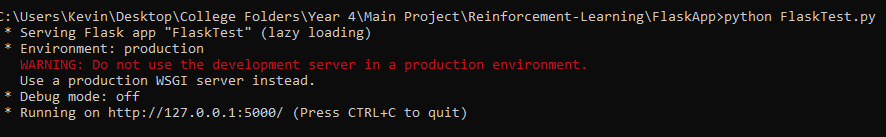
\includegraphics[width=1\linewidth]{img/flaskCmd}
	\caption{}
	\label{fig:flaskcmd}
\end{figure}
The user enters the address of http://127.0.0.1:5050 into their browser and a web page is severed from the root resource of the application with the simple message "hello world".\\\\
The following folder structure is used within a flask project.
\begin{minted}{python}
# The parent project folder
Root folder\
	# The main http routing script
	FlaskApp.py 
	# A python file that can be called
	PythonScript.py 
	# For deployment of application
	DeploymetFile.yaml
	# Declares the application python requirements at deploy time 
	RequirementsFile.txt 
	# For the staicly served files
	Static Folder\
		JavaScript Folder\
			file1.js
			filw2.js
			file3.js
		Css folder\
			style.css
		Data Folder\
			Data1.txt
			Data2.csv
			Data3.json
			Data4.xml
	# For the html templates sent back in the response body
	Templates Folder\
		home.html
		result.html
		pooling.html
\end{minted}

  
\section{REST Architecture}
The  Representational State Transfer Protocol (REST) is an architectural design philosophy that  is used to acquire resources held on a server via HTTP Requests/Responses. The REST architecture is know as stateless whereby the server holds no information about the clients session state. The session state is held locally by the client. The server only receives a client request, then sends a response back to the client with the resources requested. Resources can be in the form of text, image or html files etc. A client request is in the form of a URL with "address.com" being the physical address of the sever and "/resource-request" the actual resource needed to be sent back within the response body~\cite{Understa52:online}. 
\begin{minted}{HTTP}
https://address.com/resource-request
\end{minted} 
The main http request methods used within the REST architecture are:
\begin{itemize}
	\item GET should be used to retrieve an existing resource held on the server.
	\item POST should be used to create a resource on the server.
	\item PUT should be used to update a resource held on the server.
	\item DELETE should be used to remove a resource from the server.
\end{itemize}
Note that \textit{\textbf{should}} is used in describing the four methods above.
As the rest architecture is not a standard but rather a set of guidelines to follow, the above methods can be used for different functionality but would not be considered a restful application.
\section{JavaScript}
JavaScript is a client side browser based scripting language.
It can be used to dynamically update information on a static web page in the form of tabular data, 2D/3D animations or session based user information~\cite{JavaScri52:online}. This will be discussed further in the following subsequent subsections. JavaScript can also be used to manipulate html elements with event listeners. In the below example~\cite{fontSize:online} an onClick event listener is used to change the font size of the text contained with the html paragraph element. The element is accessed by document.getElementById('demo'). This parses the document object model DOM of the html file and locates the element with the id of 'demo'. From here  ('demo').style.fontSize='35px' alters the text style font size to 35 pixels.
This is all done dynamically via a click event on the web page allowing for the local client side real time manipulation of browser data.
\begin{minted}{HTML}
<!DOCTYPE html>
<html>
<body>

<h2>What Can JavaScript Do?</h2>

<p id="demo">JavaScript can change the style of an HTML element.</p>

<button type="button" onclick="document.getElementById('demo')
                    .style.fontSize='35px'">Click Me!</button>

</body>
</html> 
\end{minted}  
\subsection{AJAX}
Asynchronous JavaScript and XML (AJAX) is a front end browser technology wich allows for the retrieval of server side data asynchronously without altering the view or behaviour of the web page. When an asynchronous request is made to the server, it simply waits until a response has been returned and can then process the returned data. This method can be used to request specific files held on the server then run any data processing needed once the files have been returned.  AJAX also has the ability to only update partial segments of a web page without reloading the entire page.~\cite{AJAX:online}\\
In the below example~\cite{AJAXDemo:online} there is a h1 heading with the text "The XMLHttpRequest Object" along with a button holding an onClick event listener. When the button is clicked within the browser, the loadDoc() JavaScript function is called.\\
Within the loadDoc function, the onreadystatechange method waits for a http message of 4 and 200 response from the server which indicates the message has been sent correctly. From there the response text form the "ajax info" file is bound to the div with the id of demo changing the on screen text to the text held within the file.\\
 
\begin{minted}{HTML}
<!DOCTYPE html>
<html>
<body>

<div id="demo">
<h1>The XMLHttpRequest Object</h1>
<button type="button" onclick="loadDoc()">Change Content</button>
</div>

<script>
function loadDoc() {
var xhttp = new XMLHttpRequest();
xhttp.onreadystatechange = function() {
if (this.readyState == 4 && this.status == 200) {
document.getElementById("demo").innerHTML =
this.responseText;
}
};
xhttp.open("GET", "ajax_info.txt", true);
xhttp.send();
}
</script>

</body>
</html>
\end{minted}


\subsection{Google Charts}
The Google charts API is javaScript charting library that allows for the creation of numerous types of charts to be generated within a browser window. For the purpose of this project, a line chart is used to display the agent rewards gained over time. Scalable Vector Graphics (SVG) are used to render the chart image within the browser~\cite{GoogleLineChart:online}.\\
To create a line chart:
\begin{itemize}
	\item The library must be imported along with an empty div to hold the final rendered image of the chart~\cite{GoogleLineChart:online}.

\end{itemize}

\begin{minted}{HTML}
<script type="text/javascript" src="https://www.gstatic.com/charts/loader.js">
</script>
<div id="chart_div"></div>
\end{minted}
\begin{itemize}
	\item The line chart package is loaded from the library.
	\item A callback function then used to load the drawBasic() function.
\end{itemize}
\begin{minted}{JavaScript}
google.charts.load('current', {packages: ['corechart', 'line']});
google.charts.setOnLoadCallback(drawBasic);
\end{minted}
The drawBasic() function has the following elements
\begin{itemize}
	\item A data table is first instantiated to hold all of the columns, rows and data. Then columns are created with declared data types and a name. ~\cite{GoogleLineChart:online}
\end{itemize}
\begin{minted}{JavaScript}
function drawBasic() {

var data = new google.visualization.DataTable();
data.addColumn('number', 'X');
data.addColumn('number', 'Dogs');

\end{minted}
\begin{itemize}
	\item The numerical data is then added to the data table as rows. The data is represented by a two dimensional JavaScript array~\cite{GoogleLineChart:online}.
\end{itemize}
\begin{minted}{JavaScript}
data.addRows([
[0, 0],   [1, 10],  [2, 23],  [3, 17],  [4, 18],  [5, 9],
[6, 11],  [7, 27],  [8, 33],  [9, 40],  [10, 32], [11, 35],
[12, 30], [13, 40], [14, 42], [15, 47], [16, 44], [17, 48],
[18, 52], [19, 54], [20, 42], [21, 55], [22, 56], [23, 57],
[24, 60], [25, 50], [26, 52], [27, 51], [28, 49], [29, 53],
[30, 55], [31, 60], [32, 61], [33, 59], [34, 62], [35, 65],
[36, 62], [37, 58], [38, 55], [39, 61], [40, 64], [41, 65],
[42, 63], [43, 66], [44, 67], [45, 69], [46, 69], [47, 70],
[48, 72], [49, 68], [50, 66], [51, 65], [52, 67], [53, 70],
[54, 71], [55, 72], [56, 73], [57, 75], [58, 70], [59, 68],
[60, 64], [61, 60], [62, 65], [63, 67], [64, 68], [65, 69]
]);
\end{minted}

\begin{itemize}
	\item Within the options object the chart can be customised. Below names are then given to the horizontal and vertical. axis~\cite{GoogleLineChart:online}
\end{itemize}
\begin{minted}{JavaScript}
 var options = {
hAxis: {
title: 'Time'
},
vAxis: {
title: 'Popularity'
}
};

\end{minted}
\begin{itemize}
	\item Finally the container div for the chart is identified and the chart.draw method is called with the data array and personalised options as parameter arguments.~\cite{GoogleLineChart:online}
\end{itemize}
\begin{minted}{JavaScript}
      var chart = new google.visualization.LineChart(
                  document.getElementById('chart_div'));

chart.draw(data, options);
\end{minted}
This will result in a rendered line chart SVG image to the browser.~\cite{GoogleLineChart:online}

\begin{figure}[H]
	\centering
	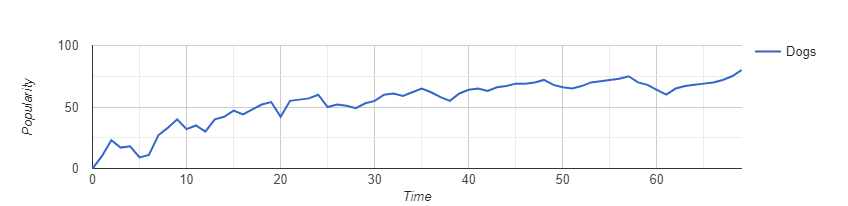
\includegraphics[width=0.7\linewidth]{img/goolgeChart}
	\caption{Goolge Line Chart}
	\label{fig:goolgechart}
\end{figure}

\subsection{Hottie heat mapping JavaScript Library}
Hottie is an open source heat mapping JavaScript library used to colour code data being generated. Any number of colour transitions can be used to represent low to high values within a dataset.The values in between low to high will have a gradient value based on the highest/ lowest value within the dataset.~\cite{HeatMap:online}\\
The hottie.js library is a used via JQuery and has the ability to colour code html tabular data based on the numerical values held within each table cell. The below example is a simple html table with some floating point values inserted into the table cells. The table has an ID of "myTable" for data access via JQuery.~\cite{HottieExample:online}
\begin{minted}{HTML}
<table id="myTable">
	<tr>
		<td>2.59</td><td>0.68</td><td>1.35</td>
		<td>1.35</td><td>2.03</td><td>1.60</td>
	</tr>
	<tr>
		<td>1.39</td><td>0.70</td><td>1.22</td>
		<td>1.08</td><td>1.00</td><td>2.12</td>
	</tr>
	<tr>
		<td>2.87</td><td>0.59</td><td>1.22</td>
		<td>0.57</td><td>1.08</td><td>3.00</td>
	</tr>
	<tr>
		<td>0.99</td><td>0.25</td><td>0.48</td>
		<td>0.50</td><td>0.99</td><td>1.77</td>
	</tr>
</table>
\end{minted}
Using JQuery, a handle is gained on the table via the ID of "myTable". Three transitional hex colour values are then set from low (red), medium (red + green) to high (green).~\cite{HottieExample:online}
\begin{minted}{JavaScript}
$("#myTable td").hottie({
colorArray : [ 
"#63BE7B",
"#FBE983",
"#F8696B"
]
});
\end{minted}
The resulting cell values within the html table now have colour codes mapped to them based on the lowest (red) to highest (green) values. Every value in between the lower and upper bound will have a mixture of the two colours. The amount of colour mix is dependant on the current value within the cell and how close it is to the lowest/highest value.~\cite{HeatMap:online}~\cite{HottieExample:online}\\
\begin{figure}[H]
	\centering
	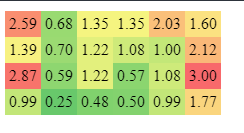
\includegraphics[width=0.7\linewidth]{img/HeatMap}
	\caption{}
	\label{fig:heatmap result}
\end{figure}

\subsection{HTML Canvas}
The html canvas element is used to draw graphics via JavaScript and render the result within a browser page.\\
All of the drawing commands are written in JavaScript and then sent to the empty canvas element for the resulting image to be rendered by the browser.\\
Below is a simple example of a line drawn using html canvas.~\cite{CanvasDoc:online}\\
The attributes the canvas element have are the with and height of the canvas view, the ID and optional styling if needed~\cite{CanvasExample:online}.

\begin{minted}{HTML}
<canvas id="myCanvas" width="200" 
           height="100" style="border:1px solid #000000;">
</canvas>
\end{minted}
To draw the line firstly, a handle is gained on the canvas element with the ID of "myCanvas".\\
The context of the canvas is then declared as a two dimensional drawing.\\
The moveTo() method tells the browser where to start the drawing with 0,0 being the x,y coordinates.
The x,y coordinates 0,0 start at the top left of the canvas which is not the conventional position of bottom left.\\
The lineTo() method states where to draw a line along the x,y coordinates. In the below example, a line is drawn 200 pixels along the x axis and 100 pixels along the y axis giving the result of a diagonal line from the top left to the bottom right of the containing canvas.~\cite{CanvasExample:online,CanvasDoc:online}
\begin{minted}{JavaScript}
var c = document.getElementById("myCanvas");
var ctx = c.getContext("2d");
ctx.moveTo(0, 0);
ctx.lineTo(200, 100);
ctx.stroke();
\end{minted}
\begin{figure}[H]
	\centering
	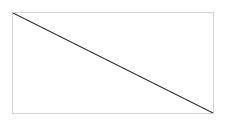
\includegraphics[width=0.7\linewidth]{img/canvasLine}
	\caption{}
	\label{fig:canvasline}
\end{figure}

\section{Bootstrap} 
Bootstrap is a CSS framework library that allows for the rapid development of a fully responsive front end user interface.\\
All css is pre-written with pre-defined class/id names.\\
To utilise the BootStrap framework, all that is required is to assign the html elements a class name or ID matching the class names or ID within the Bootstrap CSS file~\cite{Bootstrap:online}.
In the below example a simple grid layout is used by declaring three types of div with the class names of:
\begin{itemize}
	\item "container" the wrapper class that controls the responsiveness of all containing divs.
	\item "row" the class that identifies a section of the horizontal view within the browser.
	\item "col-sm" the class that identifies each column. col-sm is used in this example but the width can be set by adding a value at the end of the class name. col-sm-12 will give the column a full width of the browser window. If no numeric value is given the column width is decided by dividing the number of col class names by 12. In the below example each column is assigned a width of four as there are three divs with the class name of "col-sm".
\end{itemize} 

\begin{minted}{HTML}
<div class="container">
	<div class="row">
		<div class="col-sm">
		One of three columns
		</div>
		<div class="col-sm">
		One of three columns
		</div>
		<div class="col-sm">
		One of three columns
		</div>
	</div>
</div>
\end{minted}

The above BootStrap html will produce the following result in a browser view on a desktop at full screen~\cite{BootstrapGridExample:online}.
\begin{figure}[H]
	\centering
	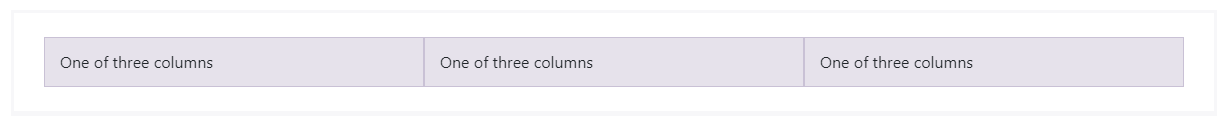
\includegraphics[width=0.7\linewidth]{img/BootstrapFullScreen}
	\caption{}
	\label{fig:bootstrapfullscreen}
\end{figure}

The below image is a view of the same BootStrap html viewed on a mobile device~\cite{BootstrapGridExample:online}.
\begin{figure}[H]
	\centering
	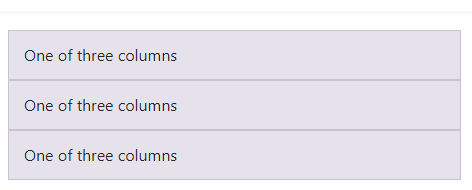
\includegraphics[width=0.7\linewidth]{img/BootstrapMobile}
	\caption{}
	\label{fig:bootstrapmobile}
\end{figure}

\section{Json}
JavaScript Object Notation (Json) is a language independent text based representation of a data object. This allows for the marshalling and un-marshalling of data to an object across many different programming languages. The Json data is written to a file with the .json extension and is usually held on a server. The .json file contents are plain text, which are interpreted by a programming language requesting the file from the server. Once the file has been received, the data can be un-marshalled to the language specific object~\cite{JSON:online}. In the below example a JavaScript object will be used to explain the process.\\

The .json file structure has  a parent container node named performance. Within this parent node there are two child nodes with key value pairs. The key for each object is named timeStep and reward with numerical values as the value for each key.~\cite{JSONstring:online}\\
\begin{minted}{JSON}
{"Performance":[
{ "timeStep":1, "reward":45 },
{ "timeStep":2, "reward":100 }
]}
\end{minted}
When the file is requested from the server, it needs to be parsed so it can be read as a JavaScript object.

\begin{minted}{JavaScript}
var obj = JSON.Parse(demo.json);
\end{minted}
The variable obj is now converted to a JavaScript object array and can be used as needed within the browser to display the relevant data.
\begin{minted}{JavaScript}
["Performance",
 [
  "timeStep"
   [
    1
   ]
 ],
 [
  "reward"
   [
    45
   ]
 ],
 [
  "timeStep"
   [
    2
   ]
 ],
 [
  "reward"
   [
    100
   ]
 ]
]
\end{minted}
\section{CSV}
A Comma Separated Value (CSV) file is used for storing data in a tabular format. Each new line within the file represents a new data entry. CSV files can be used to store multiple data types within the same file. It is then up to the program opening the file to interpret the data as needed. Below is a simple example of some numerical data entries within a csv file.~\cite{CSVPython:online} 

\begin{minted}{JavaScript}
	1,30,80,300
	2,59,67,-59
	3,40,22,21
\end{minted}

To parse this data an ajax call to a server can be used to request the file needed.~\cite{ParsingCSVExample:online}
\begin{minted}{Javascript}
$.ajax({
  type: "GET",
  url: "static/Data/test.csv",
  dataType: "text",
  cache: false,
  async: true,
  success: function(data) {
    // Array of data
    var data =data;

    $('table').append('<tr class="data"><td>'+data[0] + 
              '</td><td>'+data[1]+'</td><td>'+data[2] +
              '</td><td>'+data[3]+'</td></tr>');

  }

});
\end{minted}
In the above example once the csv file has been received from the server, the data is placed into an array and appended to a html table for rendering the data to the browser page within a table cells~\cite{ParsingCSVExample:online}.
\section{Google Cloud App Engine}
The Goolge Cloud app engine is used to deploy and host web applications to a live server.\\
In the below example a python flask application is used, however a number of different languages can be used for deployment.\\
The following requirements are needed to deploy an application to Goolge Cloud App Engine.
\begin{itemize}
	\item Create App Engine instance:
	A new project is needed as a container for the application~\cite{CreatingAppEngine:online}.
	\begin{figure}[H]
		\centering
		
\includegraphics[width=0.7\linewidth]{img/GoogleNEwPRoject}
		\caption{}
		\label{fig:googlenewproject}
	\end{figure}
	
	\item A locally created Flask project as discussed within the flask section of this chapter.
	\item app,yaml file:
	This file contains the configuration settings for the application declaring the programming language, Version number, libraries used, static directories and the main flask file name~\cite{FlaskAppGoolge:online}.
\begin{minted}{yaml}
runtime: python27
api_version: 1
threadsafe: true

libraries:
- name: ssl
version: latest

handlers:
- url: /static
static_dir: static
- url: /.*
script: main.app
\end{minted}
	\item requiremets.txt file:
	This file declares the different dependencies that are needed for the application to run.
	In the below example the flask and Werkzeug versions are declared~\cite{FlaskAppGoolge:online}.
\begin{minted}{text}
Flask==0.12.4
Werkzeug<0.13.0,>=0.12.0
\end{minted}
	\item Google Cloud SDK:
	The Google SDK must be installed locally to enable the deployment of the project to the app engine. Once the SDK has been installed open the command line tool and change to the root directory of the project folder. Once inside the directory type the following command to deploy the application~\cite{FlaskAppGoolge:online}.
\end{itemize}
\begin{figure}[H]
	\centering
	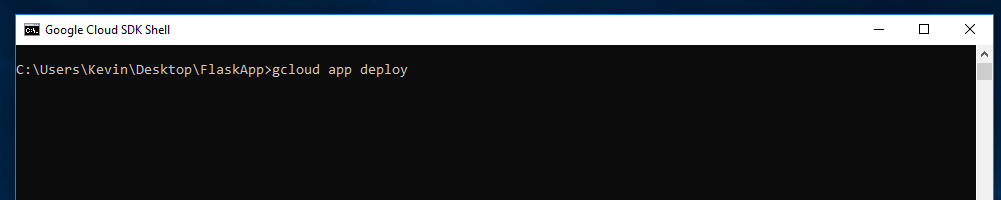
\includegraphics[width=0.7\linewidth]{img/DeployCmd}
	\caption{}
	\label{fig:deploycmd}
\end{figure}
Once the deployment has completed the application will be available at appname.appspot.com. ~\cite{FlaskAppGoolge:online}


\chapter{System Design}
This chapter will examine the overall architecture and individual system components. These will be discussed at a high level view for the main structure of the system. The major functional components will then be broken down into a more fine grain view for examination. In addition, the interaction between the components will be explained in further detail.

\section{System Architecture}
This system is client server based architecture with all of the system resources held on a server. The client interacts with the server via a resource http requests. When the client first enters the root URL of the application address, a request is made for the "Index.hmtl" web page. If found, the index page along with any other JavaScript or CSS files are sent back to the browser for rendering.

\begin{figure}[H]
	\centering
	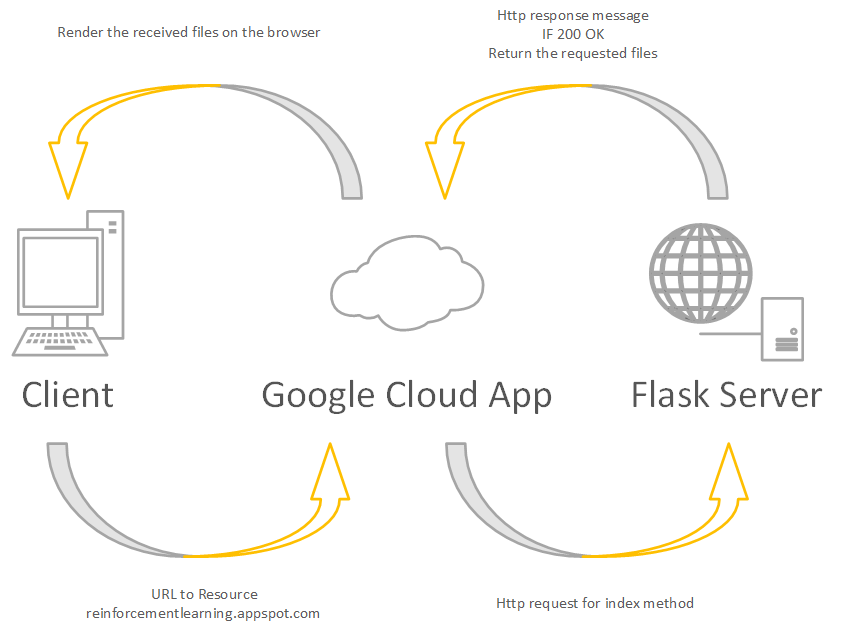
\includegraphics[width=0.7\linewidth]{img/Architecture}
	\caption{Architectural Diagram}
	\label{fig:architecture}
\end{figure}

In the following images the server will be launched locally. A request will be then sent to the server for the root resource. Finally the home page will be sent back to the browser to render the page to the user.

\begin{figure}[H]
	\centering
	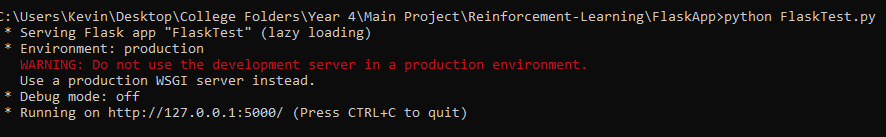
\includegraphics[width=0.9\linewidth]{img/flaskCmd}
	\caption{Starting the server}
	\label{fig:flaskcmd}
\end{figure}
The above image is the flask server running and listening for requests at http://127.0.0.1:5000/.\\
Once the URL has been entered to the address bar of the browser. 
The resource root method is called in the main Flask server file.
\begin{minted}{Python}
@app.route('/')
def index():
# Return the main home page when the route resource is requested
return render_template('index.html')
\end{minted}
The above root method returns the index.hmtl file within the response body to be read by the browser.

If everything is ok and all resources can be retrieved, a status message of 200 is sent to the browser.
\begin{figure}[H]
	\centering
	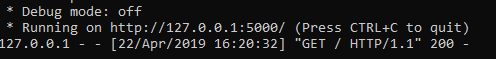
\includegraphics[width=0.9\linewidth]{img/http200}
	\caption{http 200}
	\label{fig:http200}
\end{figure}

Finally the home page is rendered to the user.
\begin{figure}[H]
	\centering
	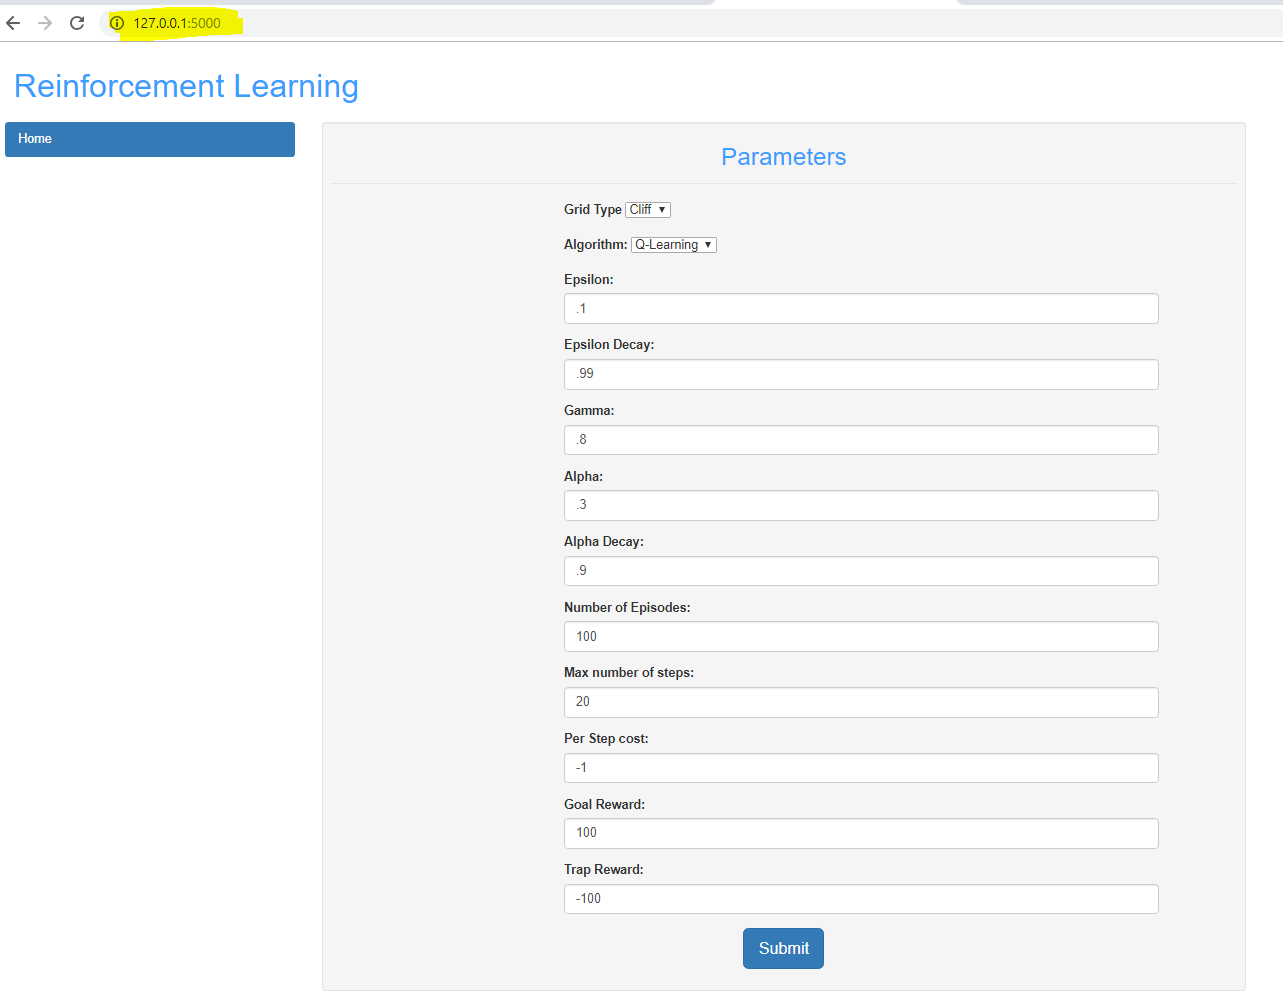
\includegraphics[width=0.9\linewidth]{img/homePage}
	\caption{Rendered Home Page}
	\label{fig:homepage}
\end{figure}
When the highlighted url is entered to the browser address, the index html page is sent back to the browser along with any CSS and JAvaScript files needed.

This example is a brief introduction of the overall architecture of the application. A more in depth investigation of each system component will be discussed in the next chapter.

\section{System Components}
The following subsections will explain how each component operates within the application.

\subsection{Environment File}
The environment.py python file holds all of the agent logic, environment space, algorithmic operations and file creation for the application.

\subsubsection{Grid Item Variables}
There are four environment objects within each grid - an agent, a trap, an empty space and the goal.
These are represented by single characters and are placed within the grids below as needed.
\begin{minted}{Python}
"""
Declare Agent, Goal, Empty and trap chars.
To be used for the environment space
"""
AGENT = 'A'
GOAL = 'G'
EMPTY = '*'
TRAP = '#'
\end{minted}
\subsubsection{Environment Grid Types}
For this application, the user can choose which grid they want to use for the agent to explore.
Below there is a grid initialised to all empty characters and a further two grids of different configurations.
\begin{minted}{Python}
"""
Initialise the initial grid with all empty variables.
"""
grid = [
[EMPTY, EMPTY, EMPTY, EMPTY, EMPTY, EMPTY],
[EMPTY, EMPTY, EMPTY, EMPTY, EMPTY, EMPTY],
[EMPTY, EMPTY, EMPTY, EMPTY, EMPTY, EMPTY],
[EMPTY, EMPTY, EMPTY, EMPTY, EMPTY, EMPTY],
[EMPTY, EMPTY, EMPTY, EMPTY, EMPTY, EMPTY],
[EMPTY, EMPTY, EMPTY, EMPTY, EMPTY, EMPTY],
]
"""
The Cliff environment.
"""
grid_cliff = [
[EMPTY, EMPTY, EMPTY, EMPTY, EMPTY, EMPTY],
[EMPTY, EMPTY, EMPTY, EMPTY, EMPTY, EMPTY],
[EMPTY, EMPTY, EMPTY, EMPTY, EMPTY, EMPTY],
[EMPTY, EMPTY, EMPTY, EMPTY, EMPTY, EMPTY],
[EMPTY, EMPTY, EMPTY, EMPTY, EMPTY, EMPTY],
[AGENT, TRAP, TRAP, TRAP, TRAP, GOAL],
]
"""
The standard environment.
"""
grid_standard = [
[EMPTY, EMPTY, EMPTY, EMPTY, EMPTY, GOAL],
[EMPTY, EMPTY, EMPTY, EMPTY, EMPTY, TRAP],
[EMPTY, EMPTY, TRAP, EMPTY, EMPTY, EMPTY],
[EMPTY, EMPTY, TRAP, EMPTY, TRAP, EMPTY],
[EMPTY, EMPTY, EMPTY, EMPTY, TRAP, EMPTY],
[AGENT, EMPTY, EMPTY, EMPTY, EMPTY, EMPTY],
]
\end{minted}

Depending on which grid the user has chosen, the empty grid gets assigned to the chosen gird.
\begin{minted}{Python}

if environment_form == "grid_cliff":
grid = grid_cliff

if environment_form == "grid_standard":
grid = grid_standard
\end{minted}
\subsubsection{State Class}
The State class is used to keep track of the agents position once the script has run.
\begin{minted}{Python}
class State:
# Initialise the class variables of grid and agent position
def __init__(self, grid, agent_pos):
self.grid = grid
self.agent_pos = agent_pos

def __eq__(self, other):
return isinstance(other, State) and self.grid == other.grid \
and self.agent_pos == other.agent_pos
\end{minted}
\subsubsection{Hyper Parameters}
The hyper parameters below are taken from the submitted form apart from the MIN ALPHA value. This value is used to ensure that the alpha value will not fall below zero when decaying after each episode.
\begin{minted}{Python}
#The max number of episodes
N_EPISODES = int(episodes_form)
# Set the maximum number of steps per episode
MAX_EPISODE_STEPS = int(max_steps_form)
MIN_ALPHA = 0.0001
# Learning rate value
alpha = float(alpha_form)
# Future reward value
gamma = float(gamma_form)  # .8
# Random action proability
eps = float(epsilon_form)  # .09
# Decay the alpha value for every completed episode
alphaDecay = float(alpha_form_decay)
# Set an array of equal values deviding alpha by the number of episodes.
alphas = np.linspace(alpha, MIN_ALPHA, N_EPISODES)
# The random action decay rate for every completed episode.
epsilon_decay = float(epsilon_form_decay)
\end{minted}
\subsubsection{Agent Actions}
The agent actions of up, down, left and right are given numerical values and placed in an array named actions. This will later be used by the choose action function.
\begin{minted}{Python}
UP = 0
DOWN = 1
LEFT = 2
RIGHT = 3
ACTIONS = [UP, DOWN, LEFT, RIGHT]

start_state = State(grid=grid, agent_pos=[5, 0])
\end{minted}
\subsubsection{Choosing Agent Actions}
This method checks if the epsilon value is greater than a randomly generated
floating point number between 0 and 1.
With the epsilon  value at .8, there is an 80\% chance of the 
agent choosing a random action.
This will force the agent to explore the environment and seek 
out all possible paths to the goal.
This values decays after each episode, gradually minimising the
chance of the agent choosing a random choice.
\begin{minted}{Python}
# Choosing an action based on the epsilon value
def choose_action(state):
if random.uniform(0, 1) < eps:
# choose a random action of up, down , left or right.
return random.choice(ACTIONS)
# If epsilon is less than the random number choosed the maximun
# value for the next state.
else:
return np.argmax(q(state))
\end{minted}
\subsubsection{Defining Agent Actions}
The below code is a snippet of a method that move the agent position. It checks the action taken of up, down left or right and moves the agent in the direction needed. 
\begin{minted}{Python}
# A deep copy of the state classs agent position to prevent
# an unwanted change in data.
p = deepcopy(state.agent_pos)
if action == UP:
# Move up and Limit the movememt to the top of the grid
p[0] = max(0, p[0] - 1)
elif action == DOWN:
# Move down and limit the movement to the bottom of the grid
p[0] = min(len(state.grid) - 1, p[0] + 1)
elif action == LEFT:
# Move left and limit the movement to the far left of the grid
p[1] = max(0, p[1] - 1)
elif action == RIGHT:
# Move right and limit the movement to the far right of the grid
p[1] = min(len(state.grid[0]) - 1, p[1] + 1)
\end{minted}
\subsubsection{Checking the agent position}
In the below code snippet, the agent position is checked for a Trap of a Goal. (Empty and Agent have been omitted for brevity). If the agent is occupying either of these grid items, a final reward is given and the episode is terminated. A new episode is started if the maximum number of episodes has not been exceeded.
\begin{minted}{Python}
# Condition to check if the grid item is a trap 
if grid_item == TRAP:
# assign the reward signal from the value set in hte form
reward = int(trap_reward)
# done to end the iteration
is_done = True
# palce the agent back to the start position
new_grid[p[0]][p[1]] += AGENT
# Check if the goal has been reached
elif grid_item == GOAL:
# assign the reward value set from the front end form
reward = int(goal_reward)
# Set the episode to done to restart another new episode
is_done = True
\end{minted}
\subsubsection{Q-Table}
The Q-Table is a dictionary that is initialised to all zero values when the script is first run.
\begin{minted}{Python}
# Q-Table dictionary
q_table = dict()
# set the state to zeros within the Q-Table
q_table[state] = np.zeros(len(ACTIONS))

\end{minted}
\subsubsection{Q-Learning Algorithm}
The Q-Learning algorithm is defined as an off policy strategy whereby the current q values are partially updated from the next state maximum q value.
With this implementation of the Q-Learning algorithm, there is an outer loop for every episode.
The inner loop is every time step for each episode.
With each iteration of the inner loop the Q-Table is updated with the Q-Learning formula~\cite{LITTMAN1994157} as discussed in chapter one\\
$Q^{new}(s_{t},a_{t})\leftarrow Q(s_{t},a_{t}) + \alpha[r_{t} + \gamma  \max _{a}Q(s_{t+1},a) - Q(s, a)]$~\cite{Qlearnin52:online}.\\ This updates the current sates value for the action taken based on the maximum value of all actions in the next state.The inner loop continues until it either reaches the maximum number of steps set by the user or a terminal state has been reached.
\begin{minted}{Python}
for e in range(N_EPISODES):
state = start_state
# Inner loop for executing every step of the agent within each episode.
for _ in range(MAX_EPISODE_STEPS):
# choose an action for each step taken
action = choose_action(state)
# assign the returned parameters from the act function
(next_state, reward, done) = act(state, action)
# assign the returned decay rate to alpha and epsilon from
# the check_terminal_state faunction
alpha, eps = check_terminal_state(done, alpha, eps)
"""
Q-Learning Algorithm
"""
# Get the max value from the next action used for updating the
# current states q value.
max_next_action = np.max(q(next_state))
# Formula for Q Learning
# Q(s, a) = Q(s, a) + alpha[r+ y * max_next_action - Q(s, a)]
# The above formula has been broken into three statements
target = reward + gamma * max_next_action
end_eq = target - q(state)[action]
q(state)[action] += alpha * end_eq
# add to total reward
total_reward += reward
# The next new stae assigned to the current state.
state = next_state
# Increment the number of steps
number_of_steps += 1
if done:
break


\end{minted}
\subsubsection{SARSA Algorithm}
The SARSA and Q-Learning algorithms look almost identical at first glance but the way in which the q values are updated are very different. The SARSA~\cite{LITTMAN1994157} algorithm $Q(s_{t},a_{t})\leftarrow Q(s_{t},a_{t})+\alpha [r_{t}+\gamma Q(s_{t+1},a_{t+1})-Q(s_{t},a_{t})]$~\cite{Stateac29:online}\\ is defined as on policy whereby its q value is partially updated based on the next state and next action, unlike Q-Learning using the maximum q value from the next state. The inner and outer loops are similar to the Q-Learning example above, with the difference being an action is chosen at the start of every episode and the next action is chosen from the next state only. The next state and next action are also updated within the inner loop~\cite{Watkins1992}. The difference in performance between the two algorithms will be examined in the next chapter.
\begin{minted}{Python}
if algorithm_form == "sarsa":
# Start the outer episode loop
for e in range(N_EPISODES):
# Get the initial start state of the agent
state = start_state
# Choose an action
# This differs from the q learning algorithm
# An action is chosen at the start of every episode
action = choose_action(state)
# Inner loop for every agent time step
for _ in range(MAX_EPISODE_STEPS):
# assign the returned parameters from the act function
(next_state, reward, done) = act(state, action)

# the next action based on the next random or max state
# This differs from q learning as the q table is update just by this action
# not the max value of all possible next actions
next_action = choose_action(next_state)
# For decaying alpha and epsilon
alpha, eps = check_terminal_state(done, alpha, eps)
# Formula for SARSA
# Q(s,a) = Q(s,a) + alpha[r + yQ(s',a') - Q(s,a)]
# Broken down into three statements
target = reward + gamma * q(next_state)[next_action]
eq_end = target - q(state)[action]
q(state)[action] += alpha * eq_end
# Set the current action to the next action
action = next_action
# set the current state to the next state
state = next_state
# add the current reward to the total reward
total_reward += reward
# increment the number of steps
number_of_steps += 1
if done:
break

\end{minted}
\subsubsection{Writing Agent Position to File}
For each step the agent takes the coordinates are written to a text file using the open python method.
\begin{minted}{Python}
completeName = os.path.join('static/Data', 'agentPos.txt')
# Open the file or create one if it doesn't exist
f = open(completeName, 'w+')
\end{minted}
From there the agent position can be written out to a text file wherever is needed using the f.write python method.

\begin{minted}{Python}
f.write('%d,' % p[0])
f.write('%d,' % p[1])
\end{minted}
As the algorithms are episodic, the agent x,y coordinates will be written out to a text file for every step the agent takes. This file can then be read via JavaScript to animate a shape representing the agent within a HTML canvas.
In addition the file will be overwritten when a new request has been made ensuring that only the latest data is present.
\subsubsection{Writing Q-Table Values to CSV File}
To store the Q-Table values as they are being generated, the dictionary holding the Q-Table is converted to a python list and then a pandas data frame. Once the Q-Table is represented as a data frame it can be converted and written to a csv file. This allows the data to be displayed within a HTML table and updated as needed. A new version of the Q-Table is appended to the csv file for every step the agent takes within the inner loop of the Q-Learning or SARSA algorithms. This supplies a complete history of every q value update as the algorithm runs. Terminal states were removed from the q table as they were all zero and of no use for the front end table data.

\begin{minted}{Python}
# check for a row in the dictionary that sums to zero
# If it does sum to zero store in empty keys
empty_keys = {k: v for k, v in q_table.items() if sum(v) == 0}
# iterate through empty_keys
for k in empty_keys:
# delete all rows with zeros
del q_table[k]
# open the Q-TAble csv file is it exits. If it doesn't exist create one.
with open('static/Data/Q_Table.csv', 'a', newline='') as f1:
#Write out and append to a dataframe the q table values
f1.write(pd.DataFrame(list(q_table.values())).to_csv(header=None))
\end{minted}
\subsubsection{Writing Rewards to Json File}
With each episode completed: 
\begin{itemize}
	\item The total rewards gained are stored in a list array
\begin{minted}{Python}
q_learning_list = []
q_learning_list.append(total_reward)
\end{minted}

	\item The list is converted to a pandas data frame
\begin{minted}{Python}
df = pd.DataFrame(q_learning_list).
\end{minted}
	\item The data frame is converted to Json
\begin{minted}{Python}
df.to_json()
\end{minted}
	\item The Json data is written out to a Json file using pandas toJson() method
\begin{minted}{Python}

with open('static/Data/q_learning.json', 'w') as al:
# write the dataframe out to a json file
al.write(df.to_json())
\end{minted}
\end{itemize}
 
\subsection{Data Files}
When the script has completed the following files are created:\\
\textbf{Q\_Learning.json:}\\
The data is structured with each episode number and total reward gained as key value pairs.
\begin{minted}{Json}
{"0":{"0":-119.0,"1":-106.0,"2":-110.0,"3":-118.0,"4":-110.0,"5":-178.0}}
\end{minted}
\textbf{Agent\_Pos.txt:}\\
Within this file, every multiple of two values represent the x, y coordinates of the agent position.
These values will be later split into tuples for animating a shape representing the agent.
\begin{minted}{JAVA}
5,0,5,0,4,0,4,0,3,0,4,0,3,0,2,0
\end{minted}
\textbf{Q\_Table.csv:}\\
The contents of this file holds the q-table values for every step the agent has taken for the duration of the chosen algorithm. The below data is the final q-table of the csv file with the state number and q values for each states action. This table is a representation of the final step the agent has taken. The file generated can be very large depending on how many episodes the user has selected. With every time step, the agent takes within each episode, a new version of the below table is appended to the csv file. Each time the script is run the file is deleted and then recreated to ensure that the latest data is only present.

\begin{table}[H]
	\hskip-2.0cm\begin{tabular}{lllll}
		State & Up & Down & Left & Right\\
		0  & 22.52511999999982   & 15.312135367563133   & 14.289668672248755   & -99.71113772079485   \\
		1  & 3.960936623865009   & 13.617460700938727   & 17.95734718463899    & 29.40639999999984    \\
		2  & -1.878271117634098  & -2.012313902784331   & -1.8815576932847637  & 15.243839125901262   \\
		3  & -1.5295742726218287 & -0.6651108864555006  & -1.453991195638845   & -1.3454791885513238  \\
		4  & -1.3298856168452398 & -1.3782276976507892  & -1.4810440112176881  & -1.4009042382447756  \\
		5  & -1.3404449880448084 & -1.236788766027146   & -1.2436143067994825  & -1.2819022725009503  \\
		6  & -1.257981734927635  & -1.3173966251263058  & -1.4462891399381745  & -1.301105125926431   \\
		7  & -1.0987670989925822 & -1.2414790942150584  & -1.125976271967187   & -0.9656125664425864  \\
		8  & -1.1551614289269732 & -0.9918947873425943  & -1.0312728318577251  & -1.0777704347717376  \\
		9  & -0.8293603632964249 & -1.0161329114408177  & -0.85828502336085    & -1.0220599125373369  \\
		10 & -0.98961            & -0.7783057291019736  & -0.7112311527378622  & -0.748887226749499   \\
		11 & -0.8319             & -0.7464912046893787  & -0.582               & -0.582               \\
		12 & -0.582              & 0.05138677455413032  & -0.8028881891543086  & -0.534987435270541   \\
		13 & -0.7853614648496994 & -0.7543131835324851  & 5.5357476588926735   & -0.7267475254392772  \\
		14 & -0.6374463101903487 & 30.48445789559959    & -0.04147787369938402 & -0.1835066667305324  \\
		15 & 6.1008142164208214  & 59.57216742404885    & 3.578987325960474    & 20.15045848281535    \\
		16 & -0.7489549628955137 & 73.3921476146162     & 14.899340036798916   & -0.49569258876485467 \\
		17 & 44.1636518774165    & 99.99999999999994    & 54.92054424745762    & 68.95364044676266    \\
		18 & -0.796333333789363  & 0.5075142332201901   & -0.7683226310600988  & -0.582               \\
		19 & -1.1213878960723254 & -1.0917344464410255  & -1.0386342926259675  & 2.0537214318666543   \\
		20 & -0.9174273822373968 & -0.34233859769154196 & -1.2038302558215905  & -0.8684927436176264  \\
		21 & -0.9418047973287629 & -1.4207538670916309  & -1.214509420128951   & -1.0517542749162405  \\
		22 & 11.488866076827776  & -99.9707299730268    & 14.315620732267625   & 38.007999999999846   \\
		23 & -1.5425145779800709 & 27.980085861161136   & 0.1955682559630758   & -1.407294795583535   \\
		24 & -1.238480339898809  & 34.474084517089224   & -1.5855723303517113  & 1.3381376892739045   \\
		25 & -1.3411399964853334 & -1.3097183035656783  & -1.1600550530407983  & -1.394592539382078   \\
		26 & 0.5247675921814534  & 7.51784556502975     & 3.8684041759256216   & 30.338944504641102   \\
		27 & 13.204714294782987  & -92.83844051173776   & 32.35995431002325    & 62.19999999999989    \\
		28 & 19.127847414768297  & -98.95976848214123   & 21.905625961034534   & 48.75999999999987    \\
		29 & -1.0351164988463812 & 2.054113774404443    & -0.6847721449750789  & 11.755097177999282   \\
		30 & 32.17905547303044   & -96.73690973090974   & 29.987489972815574   & 78.9999999999999    
	\end{tabular}
\end{table}

\subsection{index.html}:
Holds the home page with a form for the user to submit. The input fields available to the user are the choice of algorithm and hyper parameters all of which will be bound to the variables held in the environment.py file.
\begin{figure}[H]
	\centering
	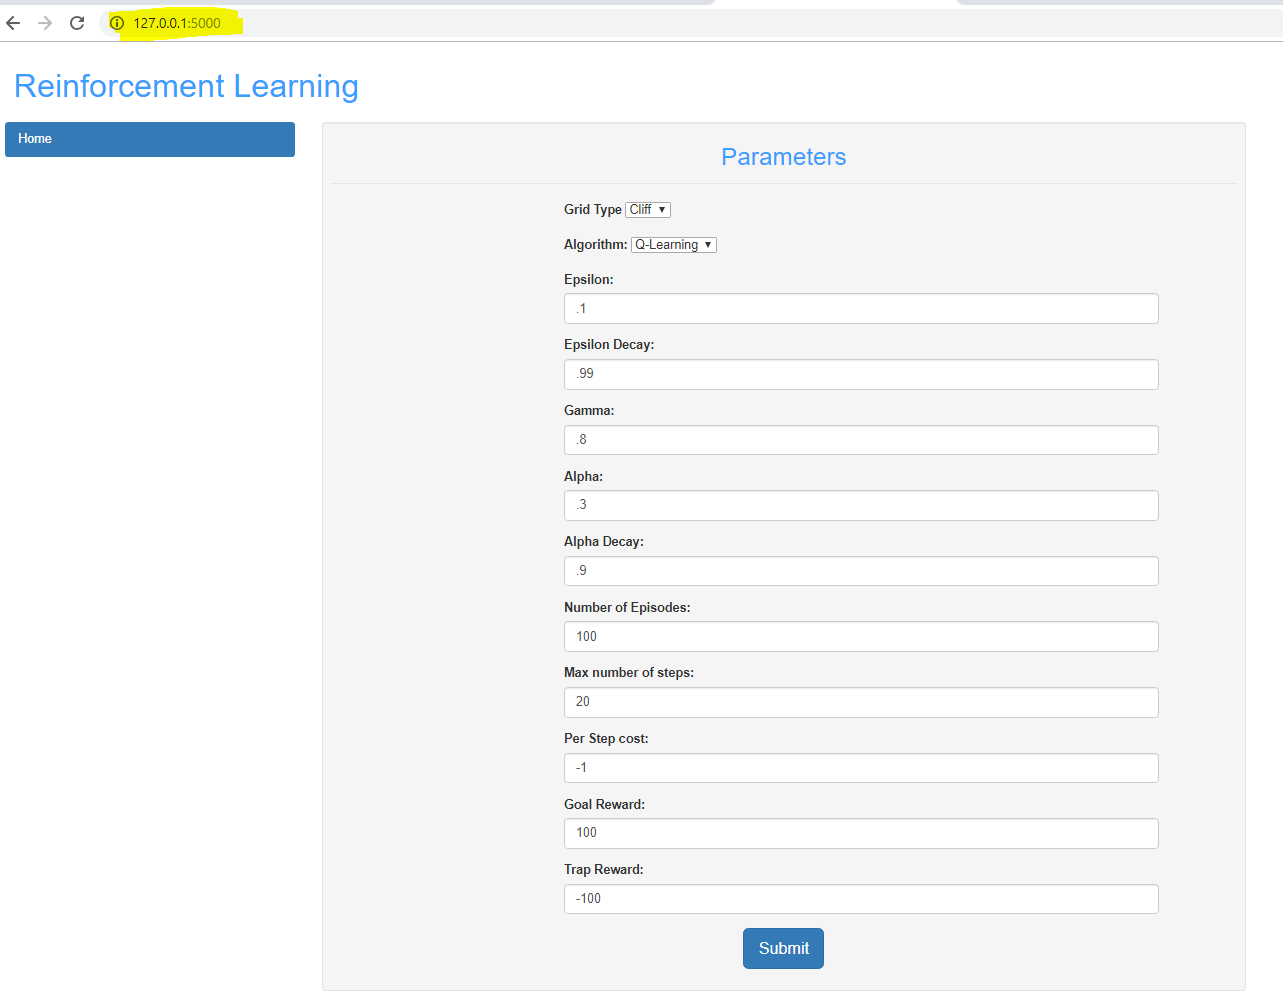
\includegraphics[width=0.7\linewidth]{img/homePage}
	\caption{}
	\label{fig:homepage}
\end{figure}
To bind the form parameters to the environment python script variables, each form input field is given an id.
\begin{minted}{html}
<input id="max_steps" name="max_steps" type="number"  min="20"
max="100" step="20" value="20" class="form-control">
\end{minted}
When the from is submitted the form data is sent as a post request and the run method is requested on the severs flask application file.
\begin{minted}{html}
<form class="form-horizontal" action="/run" method="post">
\end{minted}
Within the flask application file, the run method is called and each form input field is bound to the variables within the environment.py file. The waiting.html page is then returned to the browser for rendering.
\begin{minted}{Python}
@app.route('/run', methods=['GET', 'POST'])
def test():	
if request.method == 'POST':
environment.environment_form = request.form.get('grid_type')
environment.algorithm_form = request.form.get('algorithm')
environment.episodes_form = request.form.get('episode')
environment.max_steps_form = request.form.get('max_steps')
environment.per_step_cost = request.form.get('per_step_cost')
environment.goal_reward = request.form.get('goal_reward')
environment.gamma_form = request.form.get('gamma')
environment.epsilon_form = request.form.get('epsilon')
environment.epsilon_form_decay = request.form.get('epsilon_decay')
environment.alpha_form = request.form.get('alpha')
environment.alpha_form_decay = request.form.get('alpha_decay')
environment.trap_reward = request.form.get('trap_reward')
return render_template('waiting.html')
\end{minted}


\subsection{waiting.html}:
The waiting page simply holds an animated gif image that displays until the script has completed running.
In the background of this page, JavaScript is used to send a get request for the run resource. This will run the environment.py file and return a message of 'done' once the file has completed running.
\begin{minted}{Python}
# The first request made once teh form has been submitted
@app.route('/run', methods=['GET', 'POST'])
def test():
if request.method == 'GET':
# Call the init function from the environment.py script
environment.init()
return 'done'
\end{minted}

JavaScript is used to ping the server for a return message of "done". Once the message has been successfully returned the success resource is then requested.
\begin{minted}{JavaScript}
if (request.status === 200 && request.responseText === 'done') {
window.location = '/success';
\end{minted}
Finally the flask application file returns the result.hmtl page to the browser for rendering. In addition, the form input field values are stored in variables that can be used within template holders in the result.html page. This preserves all from data submitted by the user on the home page. This can then be inserted to the form on the result page so the user does not need to remember the original settings. This allows for the tweaking of some parameters and rerunning the application to view the difference in performance. Some of the form input variables have been omitted for brevity.
\begin{minted}{Python}
@app.route('/success', methods=['GET', 'POST'])
def dealy():
var0 = environment.environment_form
var1 = environment.algorithm_form
var2 = environment.epsilon_form
return render_template("result.html",var0=var0,var1=var1,var2=var2)
\end{minted}


\subsection{result.html}: This file displays all of the rendered data from the files generated by the environment.py file with the following UI elements.\\
The performance chart uses Google line chart JavaScript library to access the Json files via an Ajax request. There are two files requested, the SARSA and Q-Learning Json file generated by environment.py when run.
\subsubsection{Google Chart}
\begin{minted}{JavaScript}
// Make ajax call
$.ajax({
//Request the q learning json file
url: "/static/Data/q_learning.json",
dataType: "json",
// Clear cache for new data after each request
cache: false,
async: true,
success: function (data) {

var data2 = data;

$.ajax({
//Request the sarsa json file
url: "/static/Data/sarsa.json",
dataType: "json",
cache: false,
async: true,
success: function (data1) {
\end{minted}
\begin{figure}[H]
	\centering
	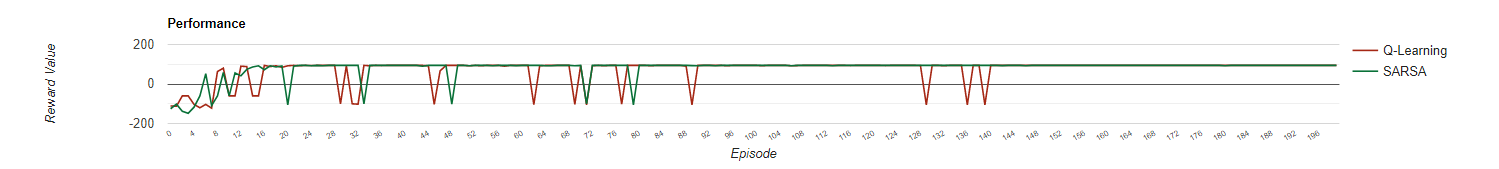
\includegraphics[width=1\linewidth]{img/performance}
	\caption{Performance Chart}
	\label{fig:performance}
\end{figure}
\subsubsection{Bootstrap framework}
The Bootstrap framework was used to style and set the layout of the page elements.
The html tags were given bootstrap id and class names to enable the forms, canvas elements and charts a responsive design. Below in a image of the result page with the from compressed to a button that will slide down when clicked. the chart and grid have also resized to fit the browser size.

\begin{figure}[H]
	\centering
	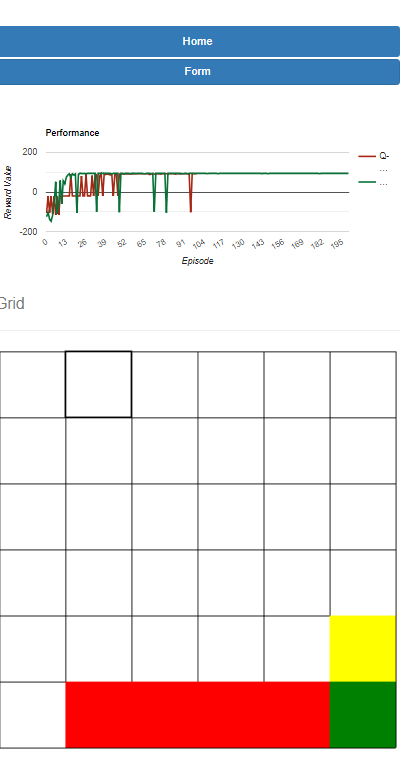
\includegraphics[width=0.7\linewidth]{img/responsive}
	\caption{}
	\label{fig:responsive}
\end{figure}



\subsubsection{Html Canvas}
The below gird environment uses the HTML canvas to animate the agent from one grid coordinate to the next. The agent position is read from the text file generated by the environment.py script.
\begin{minted}{JavaScript}
 //request the agent position text file from the server
url: "/static/Data/agentPos.txt",
dataType: "text",
cache: false,
async: true,
success: function (data)
\end{minted}
\begin{figure}[H]
	\centering
	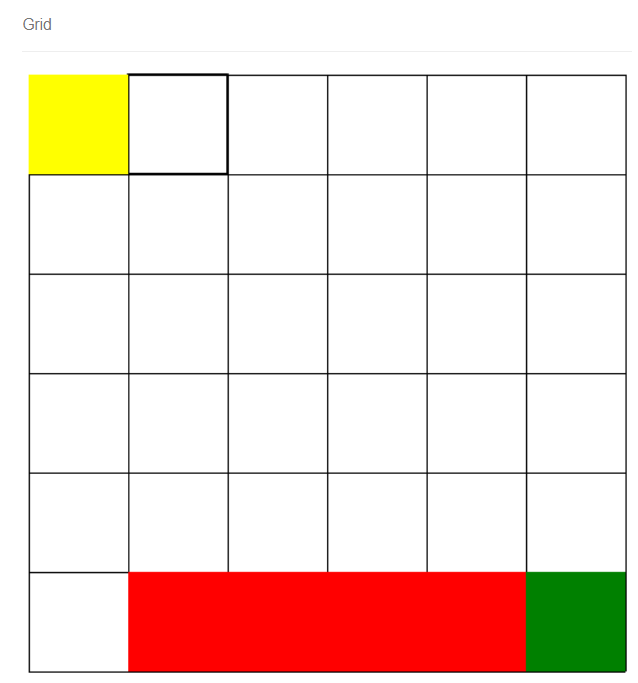
\includegraphics[width=.7\linewidth]{img/grid}
	\caption{Grid Environment}
	\label{fig:grid}
\end{figure}
Animation of the agent is achieved by a time out function where the canvas is redrawn with the agents updated position.
\begin{minted}{JavaScript}
for(let i=0; i<arr.length -2; i+=2){
// Time out function for animating the agent
window.setTimeout(function () {
// Get the x, y coordinates
x1 = arr[i];
y1 = arr[i+1];
// Clear the canvas after each frame is rendered
context.clearRect(0, 0, 650, 650);
// Call the draw board function
drawBoard();
// Check the grid type set by the form input
// Flask template variable is used to get the value in the result page
if(grid_type == "grid_standard") {
drawShape(5, 0, 'green');
drawShape(5, 1, 'red');
drawShape(4, 3, 'red');
drawShape(4, 4, 'red');
drawShape(2, 2, 'red');
drawShape(2, 3, 'red');
drawShape(y1, x1, 'yellow');
}
// Set the frame rate of hte animation
}, i * 50);
\end{minted}
\subsubsection{Q-Table Data update}
The below image of the Q-Table is populated from the Q\_Table.csv data. The file is requested via an ajax request to the server. Once the file is accessed, the data is parsed and fed to a html table. 
To update the table the data is cleared at every zero index (new q table).

\begin{figure}[H]
	\centering
	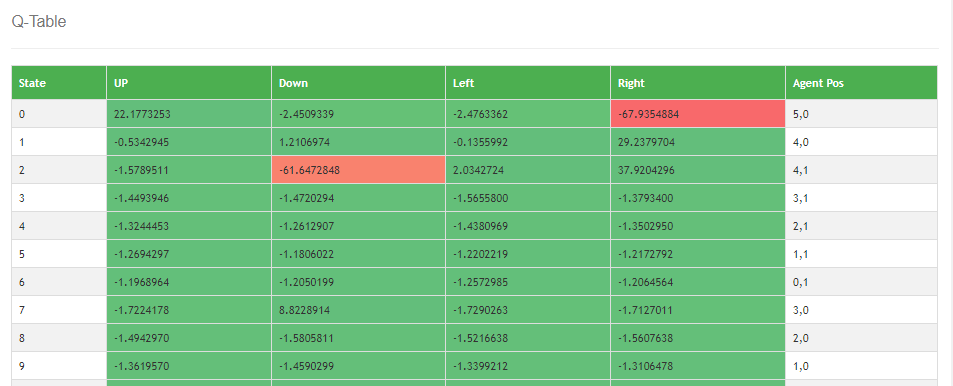
\includegraphics[width=0.7\linewidth]{img/qtable}
	\caption{Q-Table}
	\label{fig:qtable}
\end{figure}
\begin{minted}{JavaScript}
// Timeout for parsing the array of data
window.setTimeout(function () {
// Get every 5th column for each row
for(j=0; j< (result[i].length-1) / 5; j++){
// Store the 5 columns in array
csvRowCheck = result[i].slice(j * 5, (j + 1) * 5);
// Clear the data after every zero index
// Allows for updating the data after every frame
if(csvRowCheck[0]==0){
$('.data').remove();
}
// Add the data to the html table on the reult page
// Truncating the point dcimal places to 7 to save space on the page.
$('table').append('<tr class="data"><td>'+csvRowCheck[0] + 
'</td><td>'+csvRowCheck[1].toFixed(7) + 
'</td><td>'+csvRowCheck[2].toFixed(7) + 
'</td><td>'+csvRowCheck[3].toFixed(7) +
'</td><td>'+csvRowCheck[4].toFixed(7) + 
'</td><td>'+arrays[j]+ '</td></tr>');
\end{minted}
\subsubsection{Ordered Set of agent positions}
In addition, as the agent movements are randomly selected based on the epsilon value the agent position for each state will differ each time the script is run. In order to accurately map the agent position, an ordered set of x,y coordinates are needed exclusive of terminal states. This will enable the agent position for each state to be placed in the table with no repeating values. The ordering of the coordinates are not numeric, just at what point in time they have been placed in the array.\\
For example consider an array of x,y coordinates.
\begin{minted}{JavaScript}
[[0,0],[0,1],
 [0,2],[0,3],
 [0,4],[0,2],
 [0,1],[0,0],
 [1,1],[1,2],
 [2,2],[1,2]]
\end{minted}
There are un-needed repeating values of (0,0) (0,1) (0,2) and (1,2).
in order to get the unique positions the array should look like the following.\\
\begin{minted}{JavaScript}
[[0,0],[0,1],
 [0,2],[0,3],
 [0,4],[1,1],
 [1,2],[2,2]]
\end{minted}
This was achieved with JavaScript by reading the already created agent position text file. Each coordinate is split into its own array as shown in the above example. This array is then passed to a function where the JavaScript Set \{\} functionality is used. As Set behaviour has no repeating values and the converted text file of agent positions has every agent movement in order. The array can now be parsed as Json and checked as each element is placed into the JavaScript set. This now supplies a total record of unique agent positions in the order visited.
\begin{minted}{JavaScript}
// Array to hold the agent position in the q table rows
var arrays = [], size = 2;
// Ajax call for the agent position 
$.ajax({
  url: "/static/Data/agentPos.txt",
  dataType: "text",
  cache: false,
  async: true,
  success: function (data) {
    // slice the data at every ',' into and array 
    var arrt = data.split(/,/g).slice(0);
    while (arrt.length > 0) {
      /* Splice the array into gropus
       * of single array for every two x, y touples 
       */
      arrays.push(arrt.splice(0, size));
    }
    /* Function to get ordered set from the array values.
     * This will allow for the displaying of the position first
     * visited by the agent within the q table.
     * As this will change each time the program is run
     * we need a orderd set of tuples to
     * accuratley get the correct cordinates for each state visited.
     */
    function multiDimensionalUnique(arr3) {
      // Unique array
      var uniques = [];
      // set to hold unique values
      var itemsFound = {};
      // loop through the methods param input.
      for(var i = 0, l = arr3.length; i < l; i++) {
        // convert the data to json
        var stringified = JSON.stringify(arr3[i]);
        // Condition for end of data
        if(itemsFound[stringified]) { continue; }
        // put the arrays into the uniques array
        uniques.push(arr3[i]);
        // For recursive call of items found
        itemsFound[stringified] = true;
      }
      //return the unique ordered list 
      return uniques;


\end{minted}

\subsubsection{Hottie Library}
The values within the q-table are also colour coded from low (red) to high(green). This was achieved by using the Hottie JavaScript library. The table data is accessed via JQuery selectors and the cells colour is based on theses numerical values from low to high.
\begin{minted}{JavaScript}
// The Hottie framework to heatmap the values in the table as they update
// Adapted from : https://github.com/DLarsen/jquery-hottie
$("#q_table td:not(:first-child, :last-child)").hottie({
colorArray : [
"#F8696B",
"#FBE983",
"#63BE7B",
"#63BE7B",
"#63BE7B",
"#63BE7B"
]
});
\end{minted}
\subsubsection{Form Data Persistence}
The form data submitted on the home page or the result page is persisted across requests. This is achieved via flask parameter templates. \{\{var2\}\} is the second parameter returned from the success resource within the the flask application file. There are eleven other parameters that have been omitted to keep the below example concise.
\begin{minted}{HTML}
<input id="epsilon" name="epsilon" type="number" 
min="0" max="1" step=".1" 
value="{{ var2 }}" class="form-control">
\end{minted}
\begin{figure}[H]
	\centering
	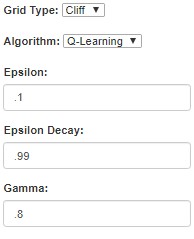
\includegraphics[width=0.7\linewidth]{img/result}
	\caption{Data kept from home page}
	\label{fig:result}
\end{figure}

\section{Sequence Digram}
\begin{figure}[H]
	\centering
	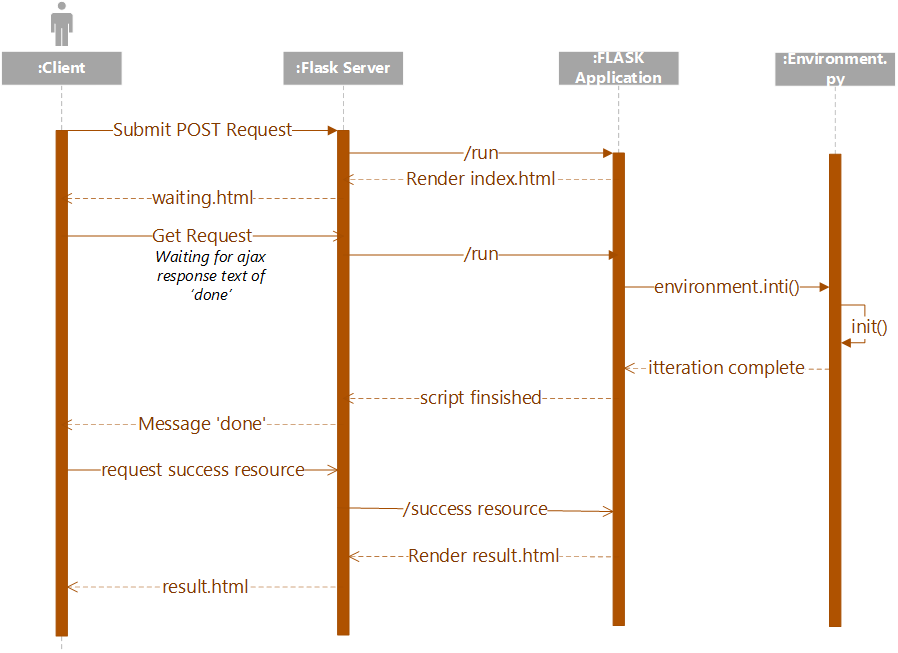
\includegraphics[width=1.2\linewidth]{img/sequence}
	\caption{}
	\label{fig:sequence}
\end{figure}


\section{Deployment}
For the deployment of a local development environment, the following two files are needed.
The files app.yaml and reqirements.txt are needed for pushing the application files to the Google application instance.

The yaml file contains the configuration information for the application including the programming language, environment type, time out limit for the server and the flask application file name.
\begin{minted}{yaml}
runtime: python
env: flex
entrypoint: gunicorn -t 120 -b :$PORT FlaskTest:app
runtime_config:
python_version: 3
\end{minted}
The requirements text file declares what python packages the application will use.
\begin{minted}{yaml}
Click==7.0
Flask==1.0.2
gunicorn==19.9.0
itsdangerous==1.1.0
Jinja2==2.10
MarkupSafe==1.1.0
Werkzeug==0.14.1
numpy==1.15.1
pandas==0.23.4
\end{minted}
Once an empty application instance has been created on Google cloud platform, the locally held files are ready to be pushed to the cloud fro deployment.\\
The Google sdk command line interface is used with the following command.

\begin{figure}[H]
	\centering
	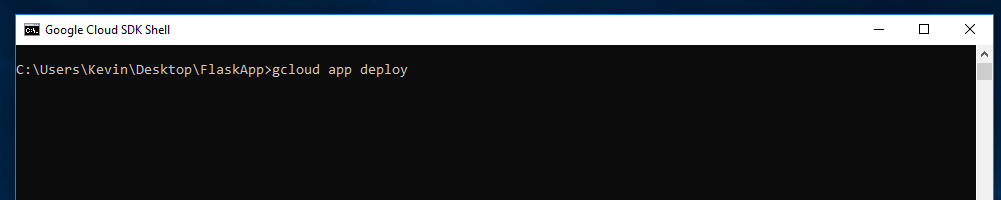
\includegraphics[width=1\linewidth]{img/DeployCmd}
	\caption{}
	\label{fig:deploycmd}
\end{figure}
Once completed the application is now live and available to anyone who wishes to access the application.



\chapter{System Evaluation}
From the objectives identified in the introduction of this document, the systems performance will be examined and documented in this chapter.
\section{Implementing SARSA and Q-learning}
The difference between the SARSA and Q-Learning algorithms should be evident once the algorithms have completed. The SARSA algorithm should take a longer path to the goal state but have less instances of falling into a negative trap state.
The environment used for this experiment is the cliff environment show below. The red squares represent traps for the yellow agent to avoid. The green square represents the goal state. Drawn on the image below is the optimal path chosen by each algorithm. The red line is the Q-Leaning optimal path chosen. The green Line is the SARSA optimal path chosen.
\begin{figure}[H]
	\centering
	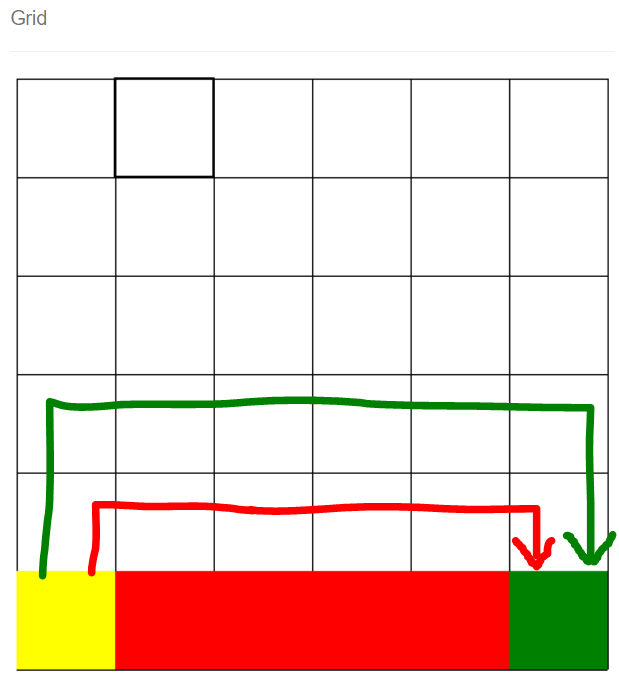
\includegraphics[width=0.7\linewidth]{img/pathOptimal}
	\caption{Paths Taken}
	\label{fig:pathoptimal}
\end{figure}

The resulting graph should show that over time q-learning gains a higher end reward per episode but has more negative trap rewards than SARSA.
Below is an image of the performance graph of both algorithms using the same input parameters.
Q-Learning is represented by the red line and SARSA by the green line.
\begin{figure}[h]
	\centering
	\includegraphics[width=1\linewidth]{"img/Q-learning eval"}
	\caption{Q-Learning reward at 94}
	\label{fig:q-learning-eval}
\end{figure}
\begin{figure}[H]
	\centering
	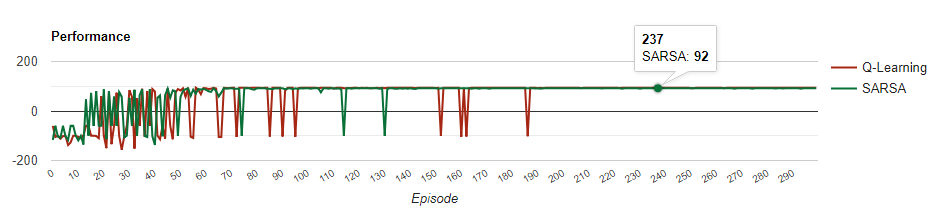
\includegraphics[width=1\linewidth]{img/SarsaEval}
	\caption{}
	\label{fig:sarsaeval}
\end{figure}

The resulting graphs show that the Q-Learning algorithm eventually gets a higher reward of 94 per episode by taking a shorter path to the goal state, resulting in an accumulative less per step penalty. However Q-learning falls into traps more frequently than SARSA.  SARSA gains an optimal reward of 92  by taking a longer path than Q-Learning this decreases the risk of randomly falling into a trap resulting in less trap terminal states than Q-learning.

\section{Flask server to handle requests}
The main Flask application file should handle resource requests as expected.\\
There are three resources declared within the application file with the following expected responses:
\begin{enumerate}
	\item The root resource of '/' should return the home page to the browser for rendering.\\
	 Result: When the root address of http://127.0.0.1:5000/ is entered to the browser address window the server responds with the message 200. The browser receives and displays the home page as expected.
	\begin{figure}[H]
		\centering
		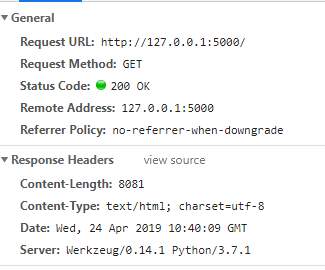
\includegraphics[width=0.7\linewidth]{img/RootReq}
		\caption{Root request}
		\label{fig:rootreq}
	\end{figure}
	
	\item The '/run' resource should accept GET and POST requests.\\
	When the form has been submitted on either the home or result pages, a POST request is made to the '/run' resource. All form field data should be bound to the environment.py variables and the waiting.html page should be returned to the browser for rendering.\\
	Result:
	\begin{figure}[H]
		\centering
		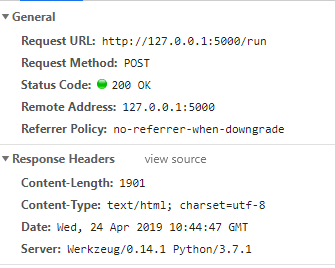
\includegraphics[width=0.7\linewidth]{img/RunResource}
		\caption{Post request /run}
		\label{fig:runresource}
	\end{figure}
	
	On the waiting.html page, an Ajax GET request should be made for the '/run' resource. This resource should then launch the environment.py script and return the response text of 'done' when the script has completed. Below in the response header the content length is 4 which represents the message 'done'\\
	Result:
	\begin{figure}[H]
		\centering
		\includegraphics[width=0.7\linewidth]{"img/Run GET"}
		\caption{Get request /run}
		\label{fig:run-get}
	\end{figure}
	
	Within the waiting.html page when a response text of 'done' has been received via ajax a new request of '/success' should be made to the server.
	Result:
	\begin{figure}[h]
		\centering
		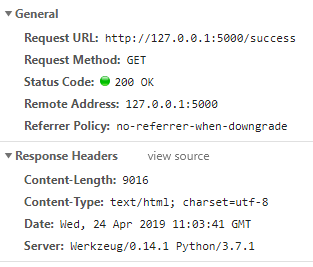
\includegraphics[width=0.7\linewidth]{img/SuccessResource}
		\caption{Get request /success}
		\label{fig:successresource}
	\end{figure}
	
	\item The '/success' resource should accept GET and Post requests.Once either request has been made it should store all of the submitted form input fields into variables so the data can be reproduced within the result page from. It should then return the result.html file along with all saved variables.\\
	Result: Below is the form submitted from the home page and then displayed on the result page with the same input data via variable binding.
	\begin{figure}[H]
		\centering
		\includegraphics[width=1\linewidth]{"img/Form home"}
		\caption{}
		\label{fig:form-home}
	\end{figure}
	\begin{figure}[H]
		\centering
		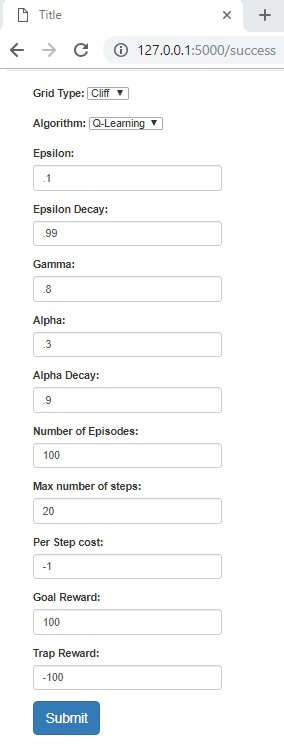
\includegraphics[width=0.7\linewidth]{img/successForm}
		\caption{}
		\label{fig:successform}
	\end{figure}
		
\end{enumerate}



\section{Ajax calls}
When the results page has been served the following files should be made available via Ajax.
\begin{enumerate}
	\item q-table.js
	\item grid.js
	\item agentChart.js
	\item agentPos.txt
	\item q-learning.json
	\item Q\_Table.csv
	\item sarsa.json
	\item styles.css
\end{enumerate}
Result:
The below images show that all of the file are being retrieved from the server as expected.
\begin{figure}[H]
	\centering
	\includegraphics[width=1\linewidth]{"img/data files"}
	\caption{}
	\label{fig:data-files}
\end{figure}
\begin{figure}[H]
	\centering
	\includegraphics[width=0.7\linewidth]{"img/Ajax files"}
	\caption{}
	\label{fig:ajax-files}
\end{figure}

\section{Agent positioning HTML canvas}
As the agentPos.txt file is read the yellow square representing the agent should correspond to each x ,y coordinate within the updating canvas.
Result:\\
Below there are two images of the first two positions the agent has taken. They are the starting position of the bottom left of the grid and a movement of one square up. The movement is behaving as expected.
\begin{figure}[H]
	\centering
	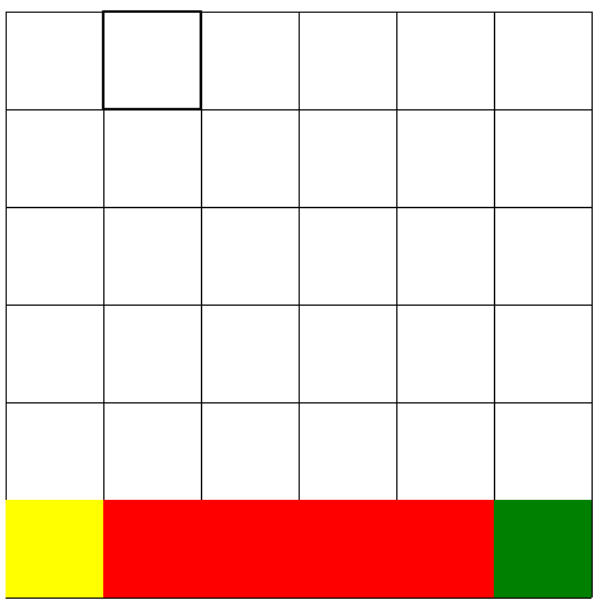
\includegraphics[width=0.7\linewidth]{img/position1}
	\caption{First Position}
	\label{fig:position1}
\end{figure}
\begin{figure}[H]
	\centering
	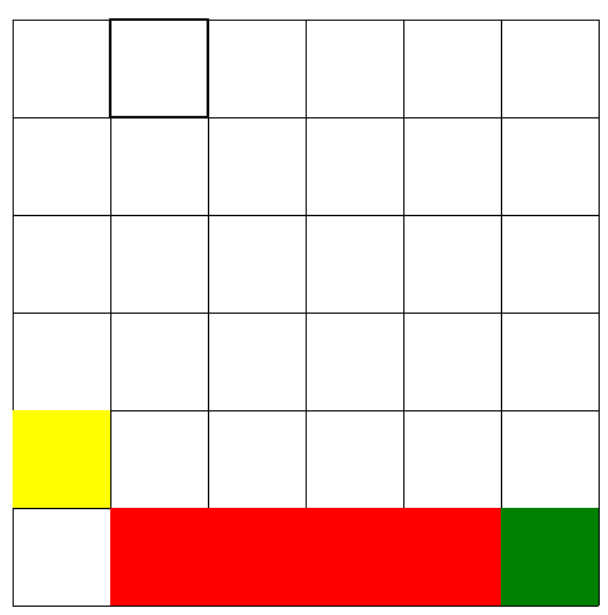
\includegraphics[width=0.7\linewidth]{img/positon2}
	\caption{Next Movement}
	\label{fig:positon2}
\end{figure}

\section{Populate table with q values}
The table present within the result.hmtl page should be populated with the q values held within the Q\_Table.csv file. As the data is populated the table should update as new values are passed to the table.\\
Result:\\
In the resulting two images below, the first image shows the initial values populating the first four rows of the table. The second image shows the updated values to the same table cells.
\begin{figure}[H]
	\centering
	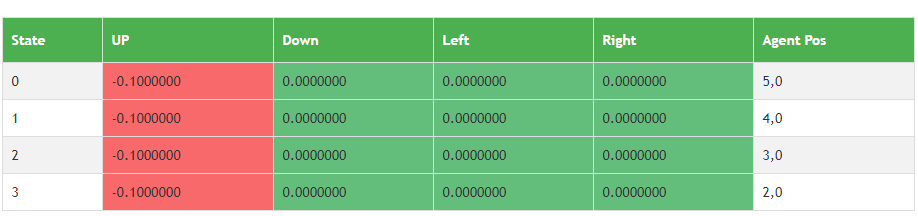
\includegraphics[width=1\linewidth]{img/Qtable1st}
	\caption{Initial Values}
	\label{fig:qtable1st}
\end{figure}
\begin{figure}[H]
	\centering
	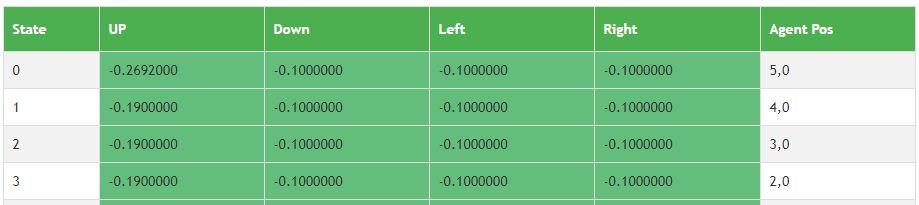
\includegraphics[width=1\linewidth]{img/QtableUpdate}
	\caption{Updated Values}
	\label{fig:qtableupdate}
\end{figure}

\section{Colour coding values of table cells}
Within the table of the result.hmtl page there are colour coded values ranging from red to green. The lowest value being red and the highest value being green. These colours are defined by the numerical values within the table cells. The table cell with the lowest value should be red and the cell with the highest value should be green. The values in between the highest and lowest value should have a transitioning gradient from red to green based on the distance between the upper and lower values held within the cells.\\
Result:\\
The Two images below is the final table split into two portions and demonstrates the colour coding working as expected.
\begin{figure}[H]
	\centering
	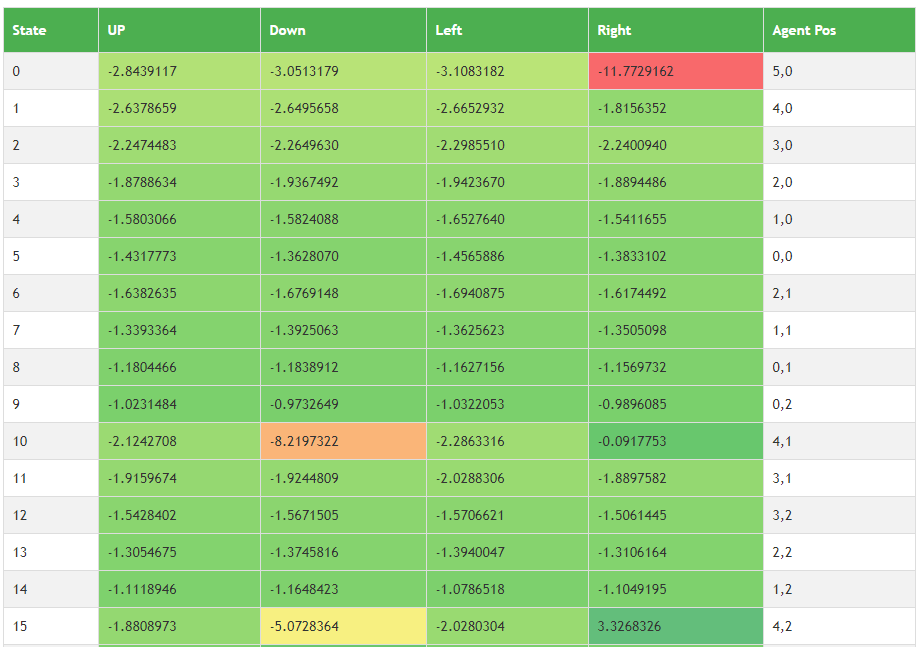
\includegraphics[width=0.7\linewidth]{img/colour1}
	\caption{Table Upper}
	\label{fig:colour1}
\end{figure}
 \begin{figure}[H]
 	\centering
 	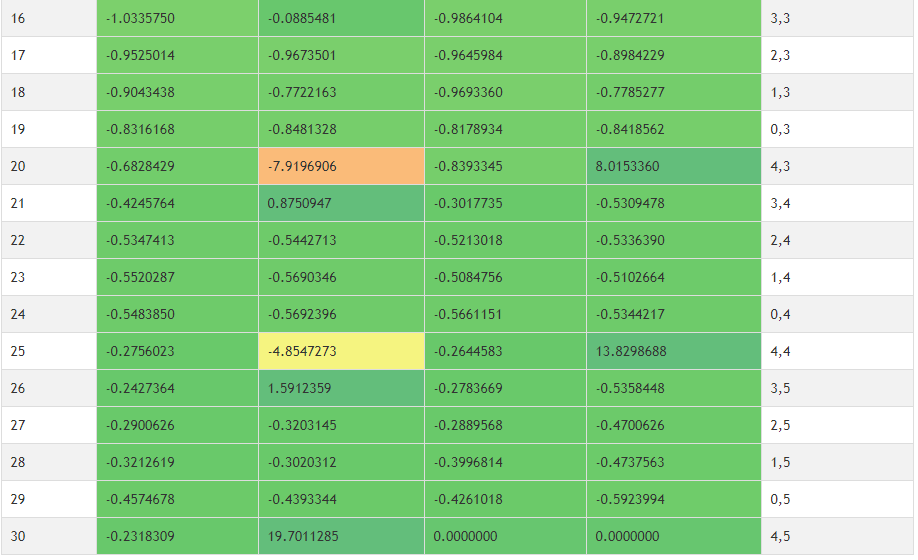
\includegraphics[width=0.7\linewidth]{img/Colour2}
 	\caption{Table Lower}
 	\label{fig:colour2}
 \end{figure}
 
\section{Google Cloud Deployment}
For the application to be fully deployed it should be available at the following URL reinforcementlearning.appspot.com.\\

Result:\\ The below images show the application live and fully working on the Google cloud platform.
\begin{figure}[H]
	\centering
	
\includegraphics[width=0.7\linewidth]{img/cloudurl}
	\caption{URL}
	\label{fig:cloudurl}
\end{figure}
\begin{figure}[H]
	\centering
	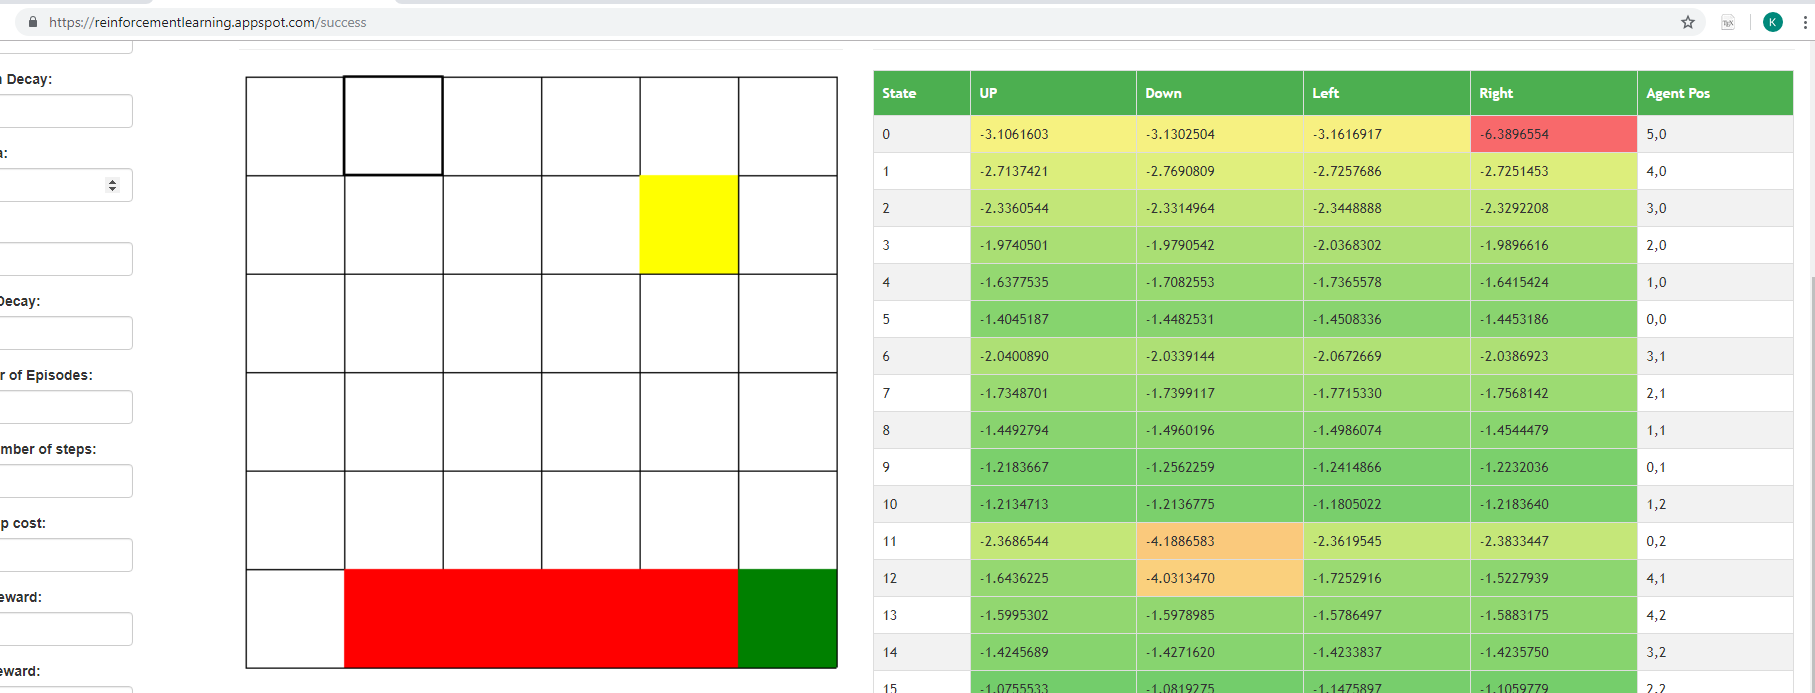
\includegraphics[width=0.7\linewidth]{img/cloudFullPage}
	\caption{Cloud Demo}
	\label{fig:cloudfullpage}
\end{figure}

\section{System Limitations}
\subsection{Appending to data frame}
While converting the Q-Table to a pandas data frame there is a significant impact on the speed the environment.py script runs. This is happening because the data frame is being appended to for every step the agent takes in each episode. For example if 1000 episodes are selected along with 100 steps per episode. There can be up to 100,000 data frames written to the csv file. The csv file can end up being approximately 30 - 40 MB in size~\cite{pandasProblem:online}.\\ This not only has an adverse effect on the speed the script runs but the load time on the browser while not detrimental can be noticeable.I had considered and tested only having the Q-Table converted for each episode which made a dramatic improvement in performance, however I decided that it is more important to have the q values update for every agent movement as this give us a deeper insight into the inner workings of the algorithm.   

\subsection{Limit in Environment size}
I would have liked to make the environment larger and more complex, but when I attempted to scale up the size of the environment it became extremely slow. With no files to write data to it could manage a reasonably large space without any problems, however this would only be a command line tool and would not have the benefit of a visual reference. 

\subsection{Agent Q-Table coordinates}
On the rare occasion the agent coordinates for a state in the q-table are incorrect. On investigating this issue I found that it had something to do with Ajax calls to two different files. The q-table gets its data from the Q\_Table.csv file and the agent position from the agentPos.txt file. They are loaded from different Ajax calls and the problem seems to be if the csv file is very large it has to wait longer than the text file with the data from the text file getting read incorrectly. As stated above this only happens on the rare occasion, while it is an issue it does not impact the application enough to be a major concern.
\subsection{Heat Map colour gradient}
When the negative and positive terminal rewards are more than a value of 50 away from each other, the colour gradient becomes less obvious. For example a negative and positive reward of -100 and 100 respectfully. The colour gradient transition is more immediate, where values between -20 and 20 there is a dramatic gradual gradient transition between the two colours. This is not a major issue rather one that has a minor impact on the visual representation of the numeric data present within the q-table.
\chapter{Conclusion}
The main purpose of this application is to provide the user with a visual aid to better understand the reinforcement learning process. The user has the ability to interact with the application via a form with inputs to change hyper parameters and a choose one of two algorithms.\\ Once the form is submitted the user will be presented with a web page that shows the agent moving within its environment, a performance chart of both algorithms along with a dynamically updating q-table.

\section{Project Outcomes}
\begin{itemize}
	\item Gained a good understanding of the python language
	\item Implementation of both SARSA and Q-Learning algorithms
	\item Breaking a complex problem set into modular units of work
	\item A Restful architecture with the Flask framework
	\item Reading and parsing different file formats via Ajax requests
	\item Generating dynamic charts from Json data
	\item Generating dynamic tables from a csv file
	\item The colour coding of HTML table data cell values
	\item Creating and animating objects with HTML Canvas
	\item Deployment of application to Google cloud platform
\end{itemize}

\section{Future Development}

In future versions of this application database integration is a real possibility. Each file generated could be stored for the retrieval of past simulations run, without the need to run the main python file.\\

There could also be a pause and step functionality where the user can stop the animations at any time and see in more detail when the decisions and values are being updated.\\

The application could be scaled out to a 3d environment with problems such as a rubix cube or 3d maze to solve. This would take a little more computing power to complete in a reasonable amount of time, but is still a problem that is achievable.\\

More algorithms could also be integrated for comparison.\\ There are, to name a few: double q-learning, deep q-learning, tensorflow integration with reinforcement learning.  Potentially any number of these could be introduced to this application for comparison.\\

\section{Final Thoughts and Acknowledgements}
\subsection{Final Thoughts}
During the development of this project, while it was challenging, I found the learning process most enjoyable. In the beginning it took a little time to research the basic concepts of reinforcement learning, but this helped greatly while later coding the algorithms needed for the application.\\
The Python programming language was also new to me, however with my prior experience of other languages, I was quickly able to pick up the basics and learn more advanced features as I needed them.\\
I particularly enjoyed working with the flask framework. I found the minimal base structure of a new application allowed for an easier understanding of how the each element is coupled.\\
In addition my experience of working with Google products has been a positive one. Prior to this project i've only had minimal experience with their cloud platform. When deploying the application and integrating line charts, their documentation quickly helped me to solve any problems I may have had.\\
In summation during the development process of this project, the overall experience has been a very positive one for me. There have been some road blocks along the way but once they were solved the end goal of the project has been even more rewarding.
\subsection{Acknowledgements}
I would like to take this opportunity to thank the following people:\\
My project supervisor Mr. Martin Hynes, who's advice and feedback given during weekly meetings was invaluable for the entire project life cycle.\\
Dr. Patrick Mannion, who gave me the original idea for the project and held a lecture on the topic which was most helpful.\\
Finally to my wife Michelle, without her understanding and support, all of this would not have been possible.\\\\
\appendix
\chapter{}
\section{GitHub Repository}
The following URL is a link to my GitHub repository holding all of the application resources.\\
\href{https://github.com/kevgleeson78/Reinforcement-Learning}{https://github.com/kevgleeson78/Reinforcement-Learning}.

\section{Installation Instruction}
You can access this application at the following URL:\\
\href{https://reinforcementlearning.appspot.com/}{https://reinforcementlearning.appspot.com/}\\

Alternatively you can clone the repository and run the application locally by following the below instructions:\\
\subsection{Local installation}
\begin{itemize}
	\item Clone the above repository using the command
\begin{minted}{bash}
git clone https://github.com/kevgleeson78/Reinforcement-Learning
\end{minted}
	\item Download and install anaconda python \href{https://www.anaconda.com/distribution/}{Click here}
	\item Open a command line tool and change directory into the FlaskApp folder of the cloned repository.
	\item Type the command "python FlaskTest.py" and press enter. This will start the server at the local address http://127.0.0.1:5000/
	\item Copy the above address into a browser window of your choice and press enter. This will now run the application within a local environment for you to interact with.
\end{itemize} 